% =============================================================================
% PolyForge — FGCS manuscript (Elsevier, elsarticle).
%
% Build (from research/paper/):   .\build.ps1
%   or: pdflatex main && bibtex main && pdflatex main && pdflatex main
%
% FGCS house rules (recorded from the Guide for Authors; the live page is
% browser-only, re-confirm on the day of submission):
%   * Abstract: concise and factual, at most 250 words, no references, no
%     undefined abbreviations; must stand alone.
%   * Keywords: 6 to 10, single concepts.
%   * Highlights: MANDATORY, separate file named "Highlights" (highlights.txt),
%     3 to 5 bullets, at most 85 characters each including spaces.
%   * Graphical abstract: optional.
%   * No page limit for regular articles.
%   * Peer review: single-anonymized (author names stay on the manuscript).
%   * Reference style: numbered, elsarticle-num.
%   * Back matter, in this order: CRediT; Declaration of competing interest;
%     Funding; Data availability; Acknowledgements; Declaration of generative
%     AI and AI-assisted technologies; References.
%   * Submission: initial = one PDF ("Manuscript"); revision = all sources in
%     ONE FLAT ARCHIVE. For the flat archive copy the used figure PDFs into
%     this directory and drop the second \graphicspath entry.
%
% Class options:
%   [preprint,review,12pt]      single column, double spaced, line numbers —
%                               the submission form.
%   [final,5p,times,twocolumn]  the journal's two-column look — length check.
%
% Sources of truth: every number in the text traces to a record under
% research/analysis/ (RESULTS_MASTER.md reconciles them). The drift gate,
% `python scripts/thesis_drift.py` from the repo root, scans this directory:
% withdrawn claims must never appear without their withdrawal beside them.
% =============================================================================
\documentclass[preprint,review,12pt]{elsarticle}

\usepackage[T1]{fontenc}
\usepackage[utf8]{inputenc}
\usepackage{lmodern}
\usepackage{graphicx}
\usepackage{booktabs}
\usepackage{tabularx}
\usepackage{longtable}
\usepackage{array}
\usepackage{amsmath,amssymb,amsthm}
\usepackage{algorithm}
\usepackage{algpseudocode}
\usepackage{tikz}
\usetikzlibrary{arrows.meta,positioning,calc}
\usepackage{xurl}
\usepackage[hidelinks]{hyperref}
\usepackage{orcidlink}
\usepackage{lineno}

\graphicspath{{figures/}{../../eval/results/figures/}}

\newcommand{\polyforge}{PolyForge}
\newcommand{\jcac}{JCAC}
\newcommand{\dz}{d_z}
\newcommand{\evfile}[1]{\texttt{#1}}
% Record file names are long and unbreakable in \texttt; let them break after
% an underscore in text (math-mode \_ is left alone).
\let\origunderscore\_
\renewcommand{\_}{\ifmmode\origunderscore\else\textunderscore\allowbreak\fi}
% Tables are single-spaced and small even under the double-spaced review option.
\newcommand{\tablefont}{\renewcommand{\baselinestretch}{1}\selectfont\small}
\newcommand{\tablefontsmall}{\renewcommand{\baselinestretch}{1}\selectfont\footnotesize}
\emergencystretch=1.5em
\newtheorem{proposition}{Proposition}

\journal{Future Generation Computer Systems}

\begin{document}

\begin{frontmatter}

\title{Per-layer optima do not compose: joint replica, semantic-cache and
model-tier control for multi-tenant AI serving, under pre-registration}

\author[ete]{Md.\ Mohaiminul Islam\corref{cor1}%
  \orcidlink{0009-0003-3254-9532}}
\ead{AUTHOR-EMAIL@example.com}          % TODO(author): institutional e-mail
\author[ete]{Farzana Akter}
\cortext[cor1]{Corresponding author.}
\affiliation[ete]{organization={Department of Electronics \& Telecommunication
  Engineering, Rajshahi University of Engineering \& Technology},
  city={Rajshahi}, postcode={6204}, country={Bangladesh}}

\begin{abstract}
Platforms that serve web traffic and AI inference for the same tenants are
steered by three controllers that never consult one another: a replica
autoscaler, a semantic response cache and a model-tier router. Each is
sound alone; whether their local optima compose had not been tested. We
built \polyforge{}, a Kubernetes-native
control plane whose planner chooses replicas, cache budget and model tier
for every tenant at once by receding-horizon optimisation of one objective
in cost, SLO violation and Jain fairness, and evaluated it under
forty-eight pre-registered protocols against baselines grid-tuned on that
objective. On the composite objective the joint controller wins in every
campaign that tested it---a 1,800-run factorial, two real demand traces, a
concurrency scaler, a 32-tenant slice and a learned controller over the
same action space---and is non-dominated in 48 of 60 cells under any
weighting. The comparative cost percentages we first obtained are
withdrawn: three pre-registered re-scorings against corrected comparators
showed they do not survive. What stands is a feasibility result: a
per-tenant budget can be kept only by a controller that holds the tier
knob. Two attempts to beat tuned reactive scalers on SLO attainment failed
and are reported as failures. On real LMSYS prompts the cache reaches
29.6\% hits at cosine 0.85, with measured precision and its ceiling;
per-tenant partitioning returns a timing side channel from AUC 0.88 to
chance, confirmed over the wire. On a rented GPU host the published
controller lost to its own tier-only ablation; a corrected controller then
beat every arm at equal fairness.
\end{abstract}

\begin{keyword}
multi-tenant serving \sep LLM inference \sep autoscaling \sep semantic caching
\sep model routing \sep model predictive control \sep SLO management
\sep cloud cost \sep pre-registration
\end{keyword}

\end{frontmatter}

\linenumbers

\section{Introduction}
\label{sec:intro}

A tenant on a modern SaaS platform issues a database read, an embedding
lookup and a chat completion inside one user-facing transaction, and the
cluster that serves all three is steered by three controllers that have
never met. A replica autoscaler---the Kubernetes Horizontal Pod Autoscaler
\citep{k8shpa}, KEDA \citep{keda} or a research successor
\citep{firm2020,sageserve2025,chiron2025,aladdin2024}---decides how much
capacity each service holds. A semantic response cache
\citep{gptcache2023,scalm2024,instcache2024,meancache2024} decides which AI
answers are served from an embedding-similarity store instead of a model
call. A model-tier router in the INFaaS tradition \citep{infaas2019} decides
which of several differently priced model classes answers each request.
Each layer has a mature literature. In every system we surveyed, each also
has its own controller: an autoscaler that has never heard of the cache, a
cache that does not know what a replica costs, a router that optimises one
request at a time.

The three layers nonetheless share one budget, one latency target and one
set of tenants, and they interact in ways none of the three controllers can
see. Growing the cache absorbs load that would otherwise demand replicas.
Escalating a tenant to a larger model raises per-request cost that a budget
must absorb, and changes the very latency signal the replica controller
scales on. A locally optimal decision at each layer can therefore be
collectively wasteful, and the waste lands on the platform's bill and on
the tenants' SLOs. This matters more every year: inference is now the
dominant line item for many platforms, model-tier prices span two orders of
magnitude, and the shift to agentic workloads---multi-step chains whose
latency is dominated by the model tier rather than by queueing---puts the
layers' interaction on the critical path.

The literature has moved toward joint decisions, but always within a layer.
Aladdin \citep{aladdin2024} co-optimises placement and scaling; horizontal
and vertical scaling have been reconciled \citep{taleoftwoscales2024}; SLO
constrained joint allocation widens a single layer's action space
\citep{jointalloc2026}; INFaaS chooses among model variants. None of these
controls a semantic cache, none carries cross-tenant fairness in its
objective, and none accounts per-tenant spend in dollars against a budget.
The 2025--26 production stack---llm-d \citep{llmd2025}, AIBrix
\citep{aibrix2025}, NVIDIA Dynamo \citep{dynamo2025}, the Gateway API
Inference Extension \citep{gatewayapi2025}---actuates on engine-level
signals (queue depth, KV-cache pressure, prefill/decode split) and leaves
the portfolio decision above it to whoever operates the cluster. Whether
per-layer optima compose into a good joint decision has, as far as we can
find, never been measured.

Our idea is to treat the three knobs as one decision. \polyforge{}'s
planner, \jcac{} (Joint Cache--Autoscaling Control), holds for every tenant
a triple---replicas, semantic-cache budget, model tier---and every ten
seconds solves one receding-horizon problem over a move-blocked action
lattice, minimising a single objective in cost, SLO violation and Jain
fairness under per-tenant budget caps and cluster caps. The solver is two
exact Gauss--Seidel sweeps over tenants; it is deterministic, runs in
microseconds, and is the same code offline and online. A Kubernetes
operator actuates the plan under guardrails.

The idea was tested rather than asserted, and we report what the test
found. Every confirmatory campaign was pre-registered: hypotheses, sole
treatment, analysis script and stopping rule were committed and pushed to a
public repository before the first run---seven protocols at the first
campaign, forty-eight by the last. The baselines were grid-tuned on our own
composite objective. On that objective the joint controller wins in every
campaign that tested it, including against an offline-trained learned
controller over the identical action space, and it is the only
Pareto-undominated system in the matrix. The evaluation also found things
we would rather not have found, and they are here at the same prominence:
two pre-registered attempts to beat tuned reactive scalers on SLO
attainment failed; the comparative cost percentages we first published were
withdrawn once an audit of the baselines found three asymmetries and three
pre-registered re-scorings showed the percentages did not survive; and on a
rented GPU host the published controller lost to its own tier-only
ablation before a corrected controller won.

What separates this work from its neighbours is compact. Against
autoscalers, it controls two knobs they do not have and prices decisions
per tenant in dollars. Against cache papers, the cache budget is a decision
variable rather than an input, and hit \emph{precision} is measured on the
same real prompts as hit rate. Against fairness schedulers, it works at the
control-plane altitude---capacity across tenants---and says so. Against
every surveyed system, it publishes its nulls under protocols frozen before
the data existed.

The paper makes the following contributions, each of which is a claim tied
to the section that carries its evidence:

\begin{itemize}
  \item \textbf{Joint cross-layer control} (Section~\ref{sec:design}). The
        first surveyed controller to co-optimise replicas, semantic-cache
        budget and model tier against one multi-tenant objective, with two
        construction-level guarantees on the deployed solver. Ablating
        jointness worsens the cost term---by $+2884\%$ against the published
        layered comparator, and by a margin 86\% smaller once that
        comparator's absorbing-tier defect is repaired; the smaller number
        is the claim (Section~\ref{sec:eval-matrix}).
  \item \textbf{A measured composition result and its adjudication}
        (Sections~\ref{sec:eval-matrix} and~\ref{sec:eval-adjudication}).
        The composite-objective win against every tuned baseline in every
        campaign; non-dominance in 48 of 60 cells; and the withdrawal of the
        like-for-like cost percentages under three pre-registered
        re-scorings, leaving a feasibility result: the per-tenant budget is
        satisfiable only by a controller holding the tier knob.
  \item \textbf{An honest SLO account} (Sections~\ref{sec:eval-slo}
        and~\ref{sec:eval-forecast}). Two confirmatory failures published as
        failures; violation parity with tuned HPA/KEDA at $-43$ to
        $-48\%$ cost; a confirmed forecasting mechanism whose winner tracks
        measured periodicity across three real traces.
  \item \textbf{Real-data cache results with a quality denominator}
        (Section~\ref{sec:eval-cache}). 29.6\% adaptive hit rate at cosine
        0.85 on LMSYS-Chat-1M, dollar-weighted savings, an empirical
        capacity curve, and---unique among surveyed cache papers---hit
        precision with the stochasticity ceiling that bounds it.
  \item \textbf{Fairness at the control-plane altitude}
        (Section~\ref{sec:eval-fairness}). Wins over a FIRM-style and a
        VTC-style baseline on Jain's index, with the controller's own
        fairness term honestly nulled.
  \item \textbf{A security frontier for shared semantic caches}
        (Section~\ref{sec:eval-security}). A timing side channel at AUC
        0.88 and a defence comparison in which per-tenant partitioning
        dominates padding and TTL jitter, confirmed at chance over the wire.
  \item \textbf{Live evidence at three depths}
        (Section~\ref{sec:eval-live}). A replica-only ordinal check that
        recorded a disagreement, a valid 24-hour soak with two of four
        hypotheses failed, a real trace driving the real cluster, and a
        three-knob live plane on which the published controller lost, the
        corrected controller won at iso-fairness, and the obvious damper
        failed.
  \item \textbf{A pre-registered systems methodology}
        (Section~\ref{sec:method}). Forty-eight protocols pushed before
        their runs, tuned baselines, paired effect sizes with bootstrap
        intervals, substrate separation, adjudication by new record rather
        than by edit, and a published ledger of nulls---a contribution that
        stands independently of any performance number.
\end{itemize}

Section~\ref{sec:threats} confronts the threats to these claims in their
strongest form, and Section~\ref{sec:conclusion} returns to each
contribution with its verdict.

\section{Related work}
\label{sec:related}

We position \polyforge{} against four bodies of work. One reading rule
applies throughout, and it is the same rule the evaluation enforces:
numbers from other papers are their numbers on their substrate---real GPU
fleets, their traces, their baselines---while ours are decision quality on
our own matrix and traces. Nothing in this section is a head-to-head cell.
Where a published system can be reproduced at simulator scale we carry it
as a tuned in-matrix baseline instead (Section~\ref{sec:method-baselines}).

\paragraph{Autoscaling for inference serving}
HPA \citep{k8shpa} and KEDA \citep{keda} are the production defaults:
reactive controllers on utilisation or event-lag signals. FIRM
\citep{firm2020} brought fine-grained, SLO-oriented resource management to
microservices. The LLM-serving generation is forecast-aware and
hierarchical. SageServe \citep{sageserve2025} reports roughly 25\% GPU-hour
savings on ten million production requests through demand forecasting;
Chiron \citep{chiron2025} reports up to $+90\%$ SLO attainment and $+70\%$
GPU efficiency through hierarchical autoscaling; Aladdin
\citep{aladdin2024} places and scales jointly for up to $-71\%$ serving
cost; an SLO-driven Kubernetes autoscaler \citep{k8sslo2025} reports
$-31\%$ violation duration at $-18\%$ cost. Horizontal-plus-vertical
scaling \citep{taleoftwoscales2024} and SLO-constrained joint allocation
\citep{jointalloc2026} widen one layer's action space; INFaaS
\citep{infaas2019} introduced model-variant selection; Faro
\citep{faro2024} targets on-premise inference clusters. Two observations
shape this paper. The systems closest to ``joint''---Aladdin, the
horizontal-plus-vertical scalers, INFaaS-style variant selection---each
co-optimise within one layer; none controls a semantic cache and none
carries cross-tenant fairness in its objective. And the published wins are
typically measured against default or non-SLO-tuned baselines, whereas
every baseline here is grid-tuned on the objective we are graded on.

\paragraph{Semantic caching}
GPTCache \citep{gptcache2023} set the pattern---embed the prompt, serve a
stored response on similarity---and reports 61.6--68.8\% hit rates on its
own benchmark. SCALM \citep{scalm2024} reports $+63\%$ hits over GPTCache;
InstCache \citep{instcache2024} pre-populates predicted instructions and
reports 51.34\% on LMSYS-Chat-1M; MeanCache \citep{meancache2024} moves the
cache to the user side; Liu et al.~\citep{semcacheadapt2025} study offline-to-online
adaptation of the similarity threshold. In all of these the cache is the
system: its size is an input, and its interaction with capacity and model
choice is out of scope. \polyforge{} treats the cache budget as one of three
jointly planned knobs, prices its benefit per tenant in dollars, and adds
two measurements the cache literature does not publish---hit precision
against the actually received response on the same real dataset
(Section~\ref{sec:eval-cache}), and a timing side channel with its defence
frontier (Section~\ref{sec:eval-security}; compare the API-layer
prompt-cache audit of Gu et al.~\citep{promptcacheaudit2025}). The eviction policy
inherits GreedyDual's inflation idea \citep{cao1997greedydual} and adds
the two terms a semantic cache needs and a proxy cache does not: staleness
under topic drift and substitutability between near-duplicate entries.

\paragraph{Multi-tenant fairness}
VTC \citep{vtc2024} defined service fairness for LLM serving at token
granularity inside a continuous-batching engine and proved a $2\times$
service bound; Equinox \citep{equinox2025}, D$^2$LPM \citep{d2lpm2025} and
Justitia \citep{justitia2025} extend it. \polyforge{}'s fairness sits at a
different altitude: capacity allocation across tenants at the control
plane, scored by Jain's index \citep{jain1984} over per-tenant SLO
satisfaction. The evaluation carries a replica-level transplant of VTC's
least-service-first rule as a tuned baseline; beating it on Jain says the
joint controller allocates capacity more evenly, not that it schedules
tokens more fairly. Token-level fair schedulers would run inside each
replica pool \polyforge{} sizes, and the two compose.

\paragraph{The 2026 serving substrate}
llm-d, AIBrix, Dynamo and the Gateway API Inference Extension actuate on
signals our system model does not name---queue depth, in-flight requests,
KV-cache pressure, prefill/decode pool split. That is an altitude
difference. \polyforge{} is the portfolio controller above that actuation
layer, and each knob has a direct target in it: replicas map to decode-pool
size or vLLM pod count, the cache budget to the gateway's semantic-cache
budget, and the tier to model routing of the kind AIBrix and INFaaS
perform. Two design decisions keep that mapping honest: the demand signal
sits behind an interface, so a token-level source (time to first token,
queue depth, KV pressure) replaces the request-rate source without touching
the planner; and latency claims stay request-level, scoped away from
continuous-batching token dynamics. What the 2026 stack does not do is
decide jointly, across a tenant portfolio, in dollars, with per-tenant
budget guardrails. That is where this work sits.

Table~\ref{tab:capability} states the four axes on which no surveyed system
overlaps with ours. The rows on which surveyed systems dominate
\polyforge{}---live GPU fleets, production scale, proven scheduling
bounds---are stated with equal care in Section~\ref{sec:threats}.

\begin{table}[htbp]
\centering\tablefont
\begin{tabularx}{\textwidth}{@{}lX@{}}
\toprule
\textbf{Axis} & \textbf{What no surveyed system does, and this one does} \\
\midrule
Architectural & co-optimise replicas, semantic-cache budget and model tier
against one multi-tenant objective \\
Economic & account per-tenant spend in dollars, with per-tenant budget
guardrails inside the controller's feasible set \\
Adversarial & publish a security evaluation of the cache layer (timing side
channel; defence frontier; over-the-wire confirmation) \\
Methodological & pre-register every confirmatory hypothesis before its run
and publish the failures at the prominence of the wins \\
\bottomrule
\end{tabularx}
\caption{The four axes that position this work. Each is a capability
statement about the surveyed literature, not a performance comparison.}
\label{tab:capability}
\end{table}

\section{Problem setting}
\label{sec:problem}

\subsection{Three knobs, one bill}

A cluster serves $m$ tenants. Each tenant's traffic is a mix of CRUD
requests and AI requests (chat completions, embeddings, agent chains), and
each tenant has an SLO expressed as a p95 latency target per traffic
class and a monthly budget expressed in dollars. Three control surfaces
determine what serving the tenant costs and how it feels:

\begin{enumerate}
  \item \emph{Replicas} $r_i$: how many instances of the serving path the
        tenant's traffic can use. Priced as infrastructure, per
        replica-hour.
  \item \emph{Semantic-cache budget} $c_i$: how much memory the gateway
        devotes to embedding-similarity lookups of past AI responses. A
        hit costs no model call; a miss costs one at the tenant's tier.
  \item \emph{Model tier} $\tau_i \in \{\text{none}, \text{small},
        \text{mid}, \text{large}\}$: which model class answers the tenant's
        AI requests. Priced per request at market API ratios of
        $1{:}10{:}100$; ``none'' is a designed AI outage that sheds AI
        requests and costs nothing.
\end{enumerate}

The knobs interact through the plant. Cache hits remove work that would
otherwise need replicas or a model call. A larger tier raises per-request
latency \emph{and} cost, and the latency it adds is exactly the signal a
utilisation-driven autoscaler reads as a need for more replicas. A budget
cap on the tenant binds on tier spend long before it binds on replica
spend: at the caps we study, tier spend dominates infrastructure spend by
three orders of magnitude (Section~\ref{sec:eval-adjudication}). A
controller that holds only one knob can therefore be locally optimal and
still make the wrong decision for the tenant's bill.

\subsection{Workload taxonomy}
\label{sec:taxonomy}

Hybrid tenants are not one workload. Over a 15-minute telemetry window we
reduce each tenant's traffic to a 12-feature vector---request rate and its
coefficient of variation, log mean payload and payload variation, mean and
p95 latency, observed cache-hit rate, mean embedding density and the
fraction of high-density prompts, mean child spans and the multi-step
fraction, and the AI-request fraction---and a softmax classifier maps the
window onto one of five classes (Table~\ref{tab:taxonomy}). Windows that
mix classes, as real tenants' windows do, are labelled by majority
composition; population-stability-index drift detection flags a tenant
whose feature distribution moves. Each class carries a control implication,
and that column is what the evaluation later makes measurable: replica-only
controllers cannot fix agentic latency because agentic latency is a tier
problem (Figure~\ref{fig:violation-by-workload}).

\begin{table}[htbp]
\centering\tablefont
\begin{tabularx}{\textwidth}{@{}l>{\raggedright\arraybackslash}p{0.44\textwidth}X@{}}
\toprule
\textbf{Class} & \textbf{Defining window statistics} & \textbf{Control implication} \\
\midrule
CRUD-steady & rate CV $\le 0.9$; mean payload $< 5$\,KB; no cache hits; no
model-tier traffic & steady replicas, minimal headroom \\
CRUD-bursty & rate CV $> 0.9$; otherwise as CRUD-steady & scale replicas
fast; no cache budget \\
AI-cacheable & model-tier traffic; embedding density $\ge 0.5$ or
high-density fraction $\ge 0.5$; observed hit rate $\ge 0.3$ & grow the
cache budget; prefer a cheap tier \\
AI-uncacheable & model-tier traffic; density $< 0.5$; hit rate $< 0.1$ &
shrink the cache; route by cost/quality \\
Agentic & mean child spans $\ge 3$ within the request's 10\,s window &
latency budget dominates; the tier knob, not replicas \\
\bottomrule
\end{tabularx}
\caption{The five-class workload taxonomy and what each class asks of the
controller. The classifier is the single implementation of these criteria;
on a held-out synthetic set of 500 contaminated windows the learned
boundary separates the classes where fixed-threshold rules do not, which
says the pipeline works and nothing yet about real traffic.}
\label{tab:taxonomy}
\end{table}

\subsection{System model and its calibration}
\label{sec:system-model}

The evaluation's decision-quality substrate is a discrete-event simulator
of this plant. Demand per tenant is aggregated to work units per second; a
congestion factor maps utilisation to latency inflation; the semantic cache
absorbs a fraction $h(c_i)\,\kappa_k$ of AI-kind $k$'s demand, with $h$ a
saturating hit-rate curve; each tier adds its base latency and its price on
every miss; replica changes and cache growth take effect with the
reconfiguration lag the realism variant bills (Section~\ref{sec:eval-slo}).
Two constants were checked against hardware before any confirmatory
campaign ran. The congestion form was fitted against a real inference
server under Poisson load: the fitted exponent ($a = 0.86$ against an
assumed $1.0$) means the model over-penalises high utilisation, which errs
against the lean postures the joint controller prefers. The tier latencies
were measured on a GPU (Table~\ref{tab:tiers}): the ordering the model
asserts holds, and the measured slope is flatter than the priced one. The
price table is a pricing assumption---bigger models run on bigger,
costlier fleets---not a hardware claim, and the matrix was re-run at the
measured corner as a sensitivity check (Section~\ref{sec:threats}). The
simulator's assumed cache curve, by contrast, turned out optimistic against
the curve later measured on real prompts; that asymmetry and its
pre-registered rerun are reported in Section~\ref{sec:threats} as well.

\begin{table}[htbp]
\centering\tablefont
\begin{tabular}{@{}llrrrr@{}}
\toprule
\textbf{Tier} & \textbf{Model} & $n$ & \textbf{mean (ms)} & \textbf{p95 (ms)} & \textbf{tokens/s} \\
\midrule
small & Qwen2.5-0.5B-Instruct & 25 & 1241.9 & 1282.7 & 38.65 \\
mid   & Qwen2.5-3B-Instruct   & 25 & 1882.8 & 1923.0 & 25.49 \\
large & Qwen2.5-7B-Instruct   & 25 & 20665.1 & 20738.0 & 2.32 \\
\bottomrule
\end{tabular}
\caption{Measured tier latencies, fixed 48-token completions, greedy
decoding, three warm-ups then 25 sequential runs per tier on a free Kaggle
GPU (\evfile{research/calibration/TIER\_BENCH.md}). The large row is an
upper bound: the 7B fp16 weights spilled to CPU on the granted card, and a
later two-GPU rerun with nothing offloaded brought it to 3171.5\,ms. An
independent replication on a fresh session reproduced every row within
3\%.}
\label{tab:tiers}
\end{table}

\section{Design}
\label{sec:design}

\polyforge{} is a control plane for multi-tenant clusters serving hybrid
workloads. We walk the loop end to end (Figure~\ref{fig:architecture}),
then give the \jcac{} formulation, the two guarantees the deployed solver
carries by construction, the cache eviction policy, and the fairness and
security decisions that the evaluation later tests.

\begin{figure}[htbp]
\centering
\resizebox{0.99\linewidth}{!}{%
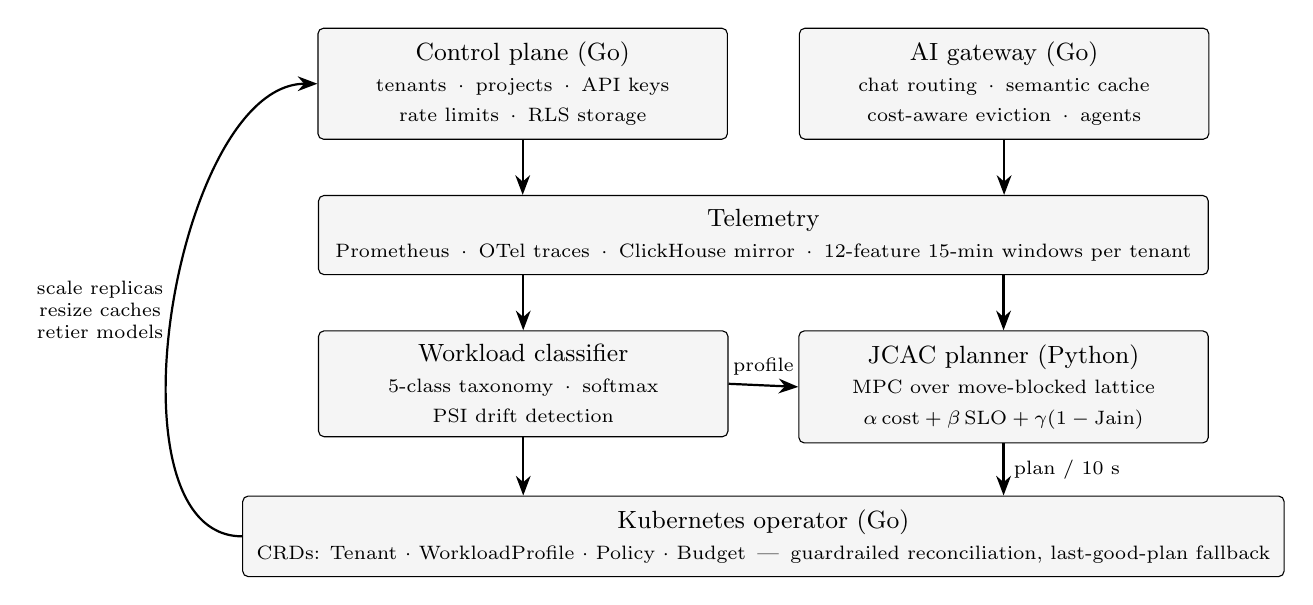
\begin{tikzpicture}[
  box/.style={draw, rounded corners=2pt, align=center, font=\small,
              minimum height=9mm, inner sep=5pt, fill=gray!8},
  arr/.style={-{Stealth[length=2.5mm]}, thick},
  node distance=7mm and 9mm
]
\node[box, minimum width=52mm] (cp)
  {Control plane (Go)\\ \scriptsize tenants \,$\cdot$\, projects \,$\cdot$\, API keys\\
   \scriptsize rate limits \,$\cdot$\, RLS storage};
\node[box, minimum width=52mm, right=of cp] (gw)
  {AI gateway (Go)\\ \scriptsize chat routing \,$\cdot$\, semantic cache\\
   \scriptsize cost-aware eviction \,$\cdot$\, agents};
\node[box, minimum width=113mm, below=of $(cp.south)!0.5!(gw.south)$] (tel)
  {Telemetry\\ \scriptsize Prometheus \,$\cdot$\, OTel traces \,$\cdot$\, ClickHouse mirror
   \,$\cdot$\, 12-feature 15-min windows per tenant};
\node[box, minimum width=52mm, below=of tel.south west, anchor=north west] (clf)
  {Workload classifier\\ \scriptsize 5-class taxonomy \,$\cdot$\, softmax\\
   \scriptsize PSI drift detection};
\node[box, minimum width=52mm, below=of tel.south east, anchor=north east] (plan)
  {\jcac{} planner (Python)\\ \scriptsize MPC over move-blocked lattice\\
   \scriptsize $\alpha\,\mathrm{cost}+\beta\,\mathrm{SLO}+\gamma(1-\mathrm{Jain})$};
\node[box, minimum width=113mm, below=7mm of $(clf.south)!0.5!(plan.south)$] (op)
  {Kubernetes operator (Go)\\ \scriptsize CRDs: Tenant $\cdot$ WorkloadProfile $\cdot$
   Policy $\cdot$ Budget \,---\, guardrailed reconciliation, last-good-plan fallback};
\draw[arr] (cp.south) -- (tel.north -| cp.south);
\draw[arr] (gw.south) -- (tel.north -| gw.south);
\draw[arr] (tel.south -| clf.north) -- (clf.north);
\draw[arr] (clf.east) -- node[above,font=\scriptsize]{profile} (plan.west);
\draw[arr] (tel.south -| plan.north) -- (plan.north);
\draw[arr] (plan.south) -- node[right,font=\scriptsize]{plan / 10 s} (op.north -| plan.south);
\draw[arr] (clf.south) -- (op.north -| clf.south);
\draw[arr] (op.west) .. controls +(-18mm,0) and +(-18mm,0) .. node[left,font=\scriptsize,align=center]{scale replicas\\ resize caches\\ retier models} (cp.west);
\end{tikzpicture}%
}
\caption{The \polyforge{} control loop. Requests (CRUD and AI, JWT-scoped
per tenant) hit the control plane and the AI gateway; per-request telemetry
is aggregated into per-tenant feature windows; the classifier labels each
tenant's workload; every 10\,s the \jcac{} planner emits a joint plan
(replicas, cache budget, model tier per tenant); the operator actuates it
under guardrails against the same data plane the requests hit.}
\label{fig:architecture}
\end{figure}

\subsection{The loop}
\label{sec:design-loop}

\paragraph{Control plane} Tenant, project and API-key management, rate
limiting, telemetry ingestion. Tenant isolation is enforced by PostgreSQL
row-level security at the database rather than in the query builder, and
it is proven by a test that queries the telemetry table with no tenant
predicate inside a tenant's transaction context and asserts that foreign
rows are invisible.

\paragraph{AI gateway} Multi-backend chat routing by plan, length and
budget; a semantic cache with cost-aware eviction
(Section~\ref{sec:eviction}); vector search; an agent loop. The cache is
per-tenant by default. That is a security decision as much as a fairness
one, and Section~\ref{sec:eval-security} shows why.

\paragraph{Telemetry and classification} Every request lands in
Prometheus metrics, OpenTelemetry traces and an analytical mirror. Per
tenant, a 15-minute window becomes the 12-feature vector of
Section~\ref{sec:taxonomy}; the classifier labels it every 10\,s and flags
drift.

\paragraph{Planner} A receding-horizon model-predictive controller over a
move-blocked action lattice (Section~\ref{sec:design-jcac}). The deployed
Python service imports the simulator's controller module, so offline
evaluation and online planning are the same code. That identity is what
licenses reading simulator decision quality as deployed decision quality.

\paragraph{Operator} Four custom resources---Tenant, WorkloadProfile,
Policy, Budget---are reconciled under guardrails: replica bounds, at most
one committed cache-level move per step, per-tenant budget caps, ordered
finalizer teardown, and last-good-plan fallback when the planner is
unreachable or over its deadline. When several Policies resolve to one
shared target, their clamped contributions are summed rather than
overwritten---a correctness property found and fixed at the desk before
the live campaign (Section~\ref{sec:impl-live}). The guardrails live in
the operator rather than the planner so that no plan source, including a
human editing a Policy object, can bypass them.

\subsection{The \jcac{} formulation}
\label{sec:design-jcac}

At each control step the planner holds tenants $T = \{1,\dots,m\}$. Tenant
$i$'s decision variable is $x_i = (r_i, c_i, \tau_i)$---replicas, cache
level, model tier---drawn from a finite per-tenant lattice $X_i$: replica
deltas $\Delta r \in \{-2,\dots,2\}$, cache moves of at most one committed
level, and any of the four tiers; hence $|X_i| \le 60$ and the joint space
$X = \prod_i X_i$ is finite. The per-step objective is
\begin{equation}
\label{eq:objective}
\begin{split}
J(x) = {}& \alpha\,\frac{1}{S}\sum_i \mathrm{cost}_i(x_i)
        + \beta \sum_i \mathrm{obj}_i(x_i)
        + \gamma \sum_i w_i \bigl(1 - \mathrm{Jain}(s(x))\bigr) \\
       & + \gamma \sum_i \nu_i\,\rho_i(x_i)
        + \lambda \sum_i \mathrm{sw}_i(x_i),
\end{split}
\end{equation}
where $\mathrm{cost}_i$ is projected dollar spend (replica-hours, cache
memory, tier price on cache misses), $\mathrm{obj}_i$ is traffic-weighted
SLO excess against the tenant's per-class p95 targets, $s(x)_i = 1 -
\mathrm{viol}_i(x_i)$ is the per-tenant SLO-satisfaction vector that enters
Jain's index \citep{jain1984}, $\nu_i$ is an exogenous interference score
from the noisy-neighbour detector, and $\mathrm{sw}_i$ counts knob switches
and supplies hysteresis. Feasibility intersects per-tenant budget caps,
$\mathrm{cost}_i(x_i) \le B_i$, with two cluster caps, $\sum_i c_i \le C$
and $\sum_i r_i \le R$; both cluster caps are separable in a scan over
tenants. Only the first action of the plan is applied before re-planning
ten seconds later. The budget cap is a hard filter: candidates that exceed
$B_i$ are rejected before the objective is evaluated, and when no candidate
is affordable the tenant is shed to tier ``none''. That design choice has
consequences the evaluation exposes twice---once as the mechanism behind a
failed risk-knob campaign, and once as the reason no replica-only
comparator can be made budget-respecting.

Demand enters through a pluggable forecaster. The code default is a linear
trend; damped Holt smoothing \citep{holt2004} is the documented recommended
default after the in-loop ablation (Section~\ref{sec:eval-slo}); an online
seasonal variant exists for streams with a detected period. The evaluation
shows the right reading is per-stream: no fixed method dominates across
three real traces, and the winner tracks measured periodicity
(Section~\ref{sec:eval-forecast}).

The solver is not a mixed-integer program. The decision variables are
integer and categorical, and with move blocking---each candidate held
across the horizon---the per-tenant lattice is small enough to enumerate
exactly. Tenants couple only through the shared sums and the satisfaction
multiset, so the planner runs two fixed Gauss--Seidel sweeps over tenants,
each block update minimising $J$ exactly over the at most 60 candidates of
one tenant with the others held fixed. The solve takes microseconds per
tenant per cycle and is deterministic, which is what makes every controller
decision in the evaluation reproducible bit for bit. An architecture
decision record explains why enumeration beat a solver dependency at this
lattice size.

\subsection{Construction-level guarantees}
\label{sec:design-theory}

Both propositions hold by construction of the deployed solver; neither is
asymptotic or probabilistic, and neither claims more than the code
delivers. Full proofs are committed with the code
(\evfile{research/analysis/THEORY\_V2.md}).

\begin{proposition}[Block-coordinate optimality]
\label{prop:bco}
Let $x^{(0)}$ be the incumbent configuration and $x^\star$ the result of
the solver's two fixed sweeps, each replacing $x_i \leftarrow
\arg\min_{x_i \in X_i(x_{-i})} J(x_i; x_{-i})$ over the feasible slice.
Then $x^\star$ is a block-coordinate minimum of $J$: no single tenant can
lower the global objective by unilaterally changing its own configuration.
\end{proposition}

\emph{Proof shape.} Each block update is an exact minimisation over a
finite set containing the incumbent, so $J$ is non-increasing across
updates. A tenant's best response depends on the others only through sums
and the satisfaction multiset, and the feasible slice depends only on
residual-cap sums, which are order-independent; a backward-propagation
argument over the last moved tenant in the second sweep shows every tenant
ends at a best response to the final configuration. $\square$

The scope is exactly the statement. A block-coordinate minimum is not the
global minimiser: the Jain coupling is non-separable, and a simultaneous
multi-tenant move could in principle beat a coordinate-wise optimum. The
gap was measured rather than assumed---the two-sweep result lands within
1\% median and 5\% maximum of an exhaustive joint optimum at every tenant
count tested (Section~\ref{sec:threats}).

\begin{proposition}[Self-calibration is bounded and contracts on agreement]
\label{prop:calibration}
Let $g_i^{(t)}$ be tenant $i$'s capacity scale under the feedback update
with learning rate $\eta = 0.15$, recovery step $\delta = 0.02$ and
tolerance $\epsilon = 0.02$. Then (a) $[0.5, 1]$ is forward-invariant and
absorbing; (b) the scale can only lower effective capacity, so planned load
is never below observed load; and (c) under sustained agreement between
projection and realisation, $g_i \uparrow 1$ in at most $\lceil 0.5/0.02
\rceil = 25$ steps and stays there.
\end{proposition}

The reading is practical: the mechanism can only make the planner more
conservative, it is confined to a bounded corrective band by explicit
projections rather than by tuning, and it relaxes back to trusting the
nominal model instead of ratcheting pessimism forever. Its empirical value
under reconfiguration realism is $\dz = +0.46$
(Section~\ref{sec:eval-slo}).

\subsection{Cost-aware semantic-cache eviction}
\label{sec:eviction}

Semantic caches gate admission by embedding similarity but evict with
classical policies---LRU or LFU---that assume every entry costs the same to
recompute. In a multi-tier gateway that is false by orders of magnitude: at
the priced tier ratios a long large-tier completion costs hundreds of times
a short small-tier one, and evicting by recency alone discards dollars.
Semantic caches also break an assumption of classical eviction analysis:
entries are not independent. Two cached prompts within the admission
threshold of each other can serve each other's hits, so evicting one of a
dense pair is nearly free while evicting an isolated entry forfeits its
future hits entirely.

Every entry $e$ therefore carries $(c_e, h_e, t^{\mathrm{store}}_e,
t^{\mathrm{last}}_e, d_e)$: recompute cost in dollars, hit count, store and
last-access times, and the similarity to its nearest cached neighbour at
store time. At eviction time $t$ each entry is scored
\begin{equation}
  w(e) = L + \underbrace{c_e}_{\text{cost}}
  \times \underbrace{\frac{h_e + 1}{1 + (t - t^{\mathrm{store}}_e)/\tau_h}}_{\text{hit rate}}
  \times \underbrace{2^{-(t - t^{\mathrm{last}}_e)/\tau_s}}_{\text{staleness}}
  \times \underbrace{\frac{1}{\varepsilon + d_e}}_{\text{isolation}}
  \label{eq:eviction-weight}
\end{equation}
and the minimum-$w$ entry is evicted (Algorithm~\ref{alg:eviction}). $L$
is the GreedyDual inflation value \citep{cao1997greedydual}, updated to the
victim's weight on every eviction, so long-resident entries must keep
re-earning their place. The hit-rate term is Laplace-smoothed so that
fresh expensive entries survive long enough to prove themselves and is
normalised by lifetime so that hoarded frequency decays---the failure mode
that sinks LFU under topic drift. The isolation term is deliberately
bounded: with $\varepsilon = 0.5$ an isolated entry outweighs a fully dense
one by at most $3\times$, so substitutability breaks ties between
economically comparable entries but never outvotes measured hit economics.
Defaults are $\tau_h = 1$\,h and $\tau_s = 6$\,h. The victim scan is $O(n)$
per eviction over per-tenant caches of $10^3$--$10^4$ entries, and the
measured p99 full-request overhead is about 1\,ms. Capacity and eviction
state are per tenant; a global budget would let one tenant's flood evict
another's expensive entries, an interference channel we verified excluded
by test. The policy's contribution in the matrix is measured by ablation
(Section~\ref{sec:eval-matrix}); its behaviour on real prompts is measured
in Section~\ref{sec:eval-cache}.

\begin{algorithm}[htbp]
\caption{Cost-aware eviction (per tenant)}
\label{alg:eviction}
\begin{algorithmic}[1]
\State \textbf{on store}$(e)$: record $(c_e, d_e)$;
  $h_e \gets 0$; $t^{\mathrm{store}}_e, t^{\mathrm{last}}_e \gets \text{now}$
\State \textbf{on hit}$(e)$: $h_e \gets h_e + 1$;
  $t^{\mathrm{last}}_e \gets \text{now}$
\While{$|\text{cache}| > \text{capacity}$}
  \State $v \gets \arg\min_{e} w(e)$
    \Comment{Eq.~\eqref{eq:eviction-weight}, $O(n)$ scan}
  \State $L \gets w(v)$; evict $v$
\EndWhile
\end{algorithmic}
\end{algorithm}

\subsection{Fairness and security in the design}
\label{sec:design-fairsec}

The noisy-neighbour detector scores tenants peer-relatively on
eBPF-shaped signals, and the score enters the objective as the
$\nu_i\rho_i$ penalty; Jain's index over SLO satisfaction is exported
every cycle. The $\gamma$-weighted Jain term is a design feature whose
measured contribution under injected interference turned out to be a null
(Section~\ref{sec:eval-fairness}); it stays configurable, and the fairness
claims rest on measured outcomes rather than on the term's presence.

Sharing a semantic cache across tenants opens a timing side channel: a hit
on a prompt another tenant inserted returns faster, and response time
alone leaks membership. The design defence is per-tenant partitioning with
demand-proportional sizing. The evaluation quantifies both the attack and
the frontier of defences (Section~\ref{sec:eval-security}); the
per-tenant default in the gateway is the consequence of that measurement,
not a prior.

Every architectural choice with a live alternative is recorded as a
decision record in the repository (\evfile{docs/adr/}). The load-bearing
ones are row-level security at the database rather than the query
builder, enumeration rather than a MIP backend for the planner, and
peer-relative rather than absolute noisy-neighbour detection.

\section{Implementation}
\label{sec:impl}

\polyforge{} is a working system, not a simulator with a paper around it.
This section records what was built, the gates it is held to, and the two
defects that wiring the live evaluation arm surfaced before any cluster
time was spent.

\paragraph{Components} The control plane (Go; \evfile{cmd/control-plane},
\evfile{internal/}) exposes tenant, project and API-key APIs over
PostgreSQL with row-level security (an SQLite path exists for
development), rate limiting, telemetry ingestion, and canary and
isolation-ladder admin APIs. The AI gateway (Go; \evfile{cmd/ai-gateway},
\evfile{internal/ai}) routes chat across backends by plan, length and
budget, and hosts the semantic cache, vector search and the agent loop.
The classifier (\evfile{internal/classifier}, trained by
\evfile{cmd/classifier-train}) turns 12-feature windows into taxonomy
labels every 10\,s with PSI drift detection. The \jcac{} planner
(\evfile{services/planner}) imports the simulator's controller from
\evfile{research/jcac\_sim}, so offline and online planning are one code
path. The operator (Go; \evfile{cmd/operator}, Helm chart under
\evfile{deploy/helm}) reconciles the four custom resources with the
guardrails of Section~\ref{sec:design-loop}, tears down in finalizer
order, and traces every reconcile. The evaluation harness (\evfile{eval/})
is YAML-driven, carries the tuned baselines, writes DuckDB results, and
has a kind-cluster live backend.

\paragraph{Engineering gates} Every change passes the same battery before
commit: \texttt{gofmt}, \texttt{go vet}, \texttt{go build}, \texttt{go
test ./... -count=1} across 26 Go packages, the Python suites for the
harness, planner and analysis, and OpenAPI linting. Continuous integration
additionally runs the race detector, a coverage gate, golangci-lint and the
row-level-security suite against a live PostgreSQL service. Tests that only
CI can execute are reported as unproven until a green CI run, and the
session log records how every change was verified. Security-relevant
details received the treatment of research claims: API-key identifiers are
drawn independently of the secret after an audit found the identifier
leaked 64 of 192 entropy bits; keys are hashed with SHA-256 rather than
argon2id, sound because the secrets are 192-bit random strings, and
recorded as a deliberate deviation precisely because it invites the
question; a recovery middleware returns structured errors without stack
details; the authentication packages are held at roughly 95\% coverage.

\paragraph{Deviations from the original plan} Three tools named in the
original roadmap were replaced with equivalent outcomes and the
replacement recorded rather than silently made: the chi router by Go
1.22's standard-library method patterns; sqlc and golang-migrate by
hand-written SQL behind repository interfaces plus an idempotent migrator
(type-safe access and a versioned schema still hold, and row-level
security is proven by test); argon2id by SHA-256 as above. The evaluation
reports latency at p95 rather than the roadmap's p99, for a reason
Section~\ref{sec:method-metrics} gives.

\subsection{The live arm, and two defects found at the desk}
\label{sec:impl-live}

The live campaigns (Section~\ref{sec:eval-live}) run on a kind cluster
with harness-built images, a k6 load generator, real HPA for the baseline
arm, and the operator plus planner for the \jcac{} arm. Wiring that arm
surfaced two defects, each of which would have silently invalidated a
cluster session.

The first was demand plumbing that could never have authenticated. The
operator's feature-demand source sent its token as a bearer, which the
control plane treats strictly as a JWT; every read would have returned
401, and because the \jcac{} loop degrades by design into silent fallback,
the arm would have run ``live'' while planning nothing. The features
endpoint---that endpoint only---now accepts the platform admin key, and
the change is unit-tested in both directions: the admin key reads any
tenant's features and still cannot touch other tenant routes.

The second was last-writer-wins actuation on a shared target. All eight
evaluation tenants' Policies name one shared Deployment, and each
reconcile overwrote the others' replica counts, which would have pinned
the target at a single tenant's share---the joint controller crippled by
wiring and labelled as the joint controller. Policies that resolve to the
same target now sum their clamped contributions, deletion re-enqueues the
siblings, and the behaviour is unit-tested.

Both fixes travel with a more general honesty mechanism. The harness ends
operator installation with \texttt{kubectl wait --for=condition=Applied}
on every Policy, so a run in which the operator never actuated fails
before any load is generated; ``the controller was actually in the loop''
is an executable gate rather than a promise. Capacity parity is a cell
property under test: every arm starts at the same replica count and is
ceilinged by the same cluster limits, so no arm can win by being handed
more cluster.

\subsection{Scale behaviour of the deployed planner}
\label{sec:impl-scaling}

The deployed \texttt{PlannerCore.plan} path was driven from 8 to 256
tenants on one laptop core. The fitted growth exponent is 1.45: the joint
fairness term couples tenants, and super-linearity is the measured price of
jointness. The p95 cycle time first exceeds the operator's 3\,s request
timeout at 128 tenants and the 10\,s control period at 256. Past the
timeout the failure mode is the designed one---the operator holds the last
good plan and reports fallback status. The levers past the crossover were
then measured rather than named: hash-based planning cells hold the
per-cell p95 under the timeout through 1,024 tenants, at a global-Jain
cost the first cell assignment exceeded and a de-aliased assignment brings
within bound; the wall reproduces at the same width through the shipped Go
operator (Section~\ref{sec:threats}). Coordination costs outside the
planner---custom-resource write fan-out, telemetry aggregation---are not
covered by this microbenchmark.

\section{Methodology}
\label{sec:method}

The credibility of what follows rests on rules that were fixed before any
result existed. We state them here; Section~\ref{sec:eval} reports what
happened under them, including the hypotheses that failed.

\subsection{Pre-registration}
\label{sec:method-prereg}

Every confirmatory campaign's protocol---hypotheses, sole treatment,
analysis script and stopping rule---was committed and pushed to the public
repository before its first run, in the spirit of the pre-registration
practice that other empirical fields adopted a decade ago
\citep{nosek2018prereg}. Forty-eight such protocols exist, each anchored by
its push timestamp; all are mirrored, frozen and public with a DOI on the
Open Science Framework, a mirror made after the campaigns ran and stated
as such. A gate script proves from the git history that no registered text
was altered after its result existed. Protocol changes forced by
feasibility---the LMSYS similarity matrix that would not fit in 40\,TB, for
one---were committed as declared pre-run amendments before the gated data
was downloaded; the amendment chain is the registration's continuation and
is visible in the history. Closed campaigns are immutable: stopping rules
forbid re-running, widening or post-hoc tuning, and a campaign's result
file is never edited after its run. When a confound was found after a
campaign had closed---three were, in an audit of the baseline
implementations---the response was a new pre-registration whose outcome
for the published claim was committed before the re-scoring ran, and a new
record beside the old one. The published record stands; the paper quotes
the surviving claim. Figure~\ref{fig:evidence-flow} is the path every
number in this paper took.

\begin{figure}[htbp]
\centering
\resizebox{0.99\linewidth}{!}{%
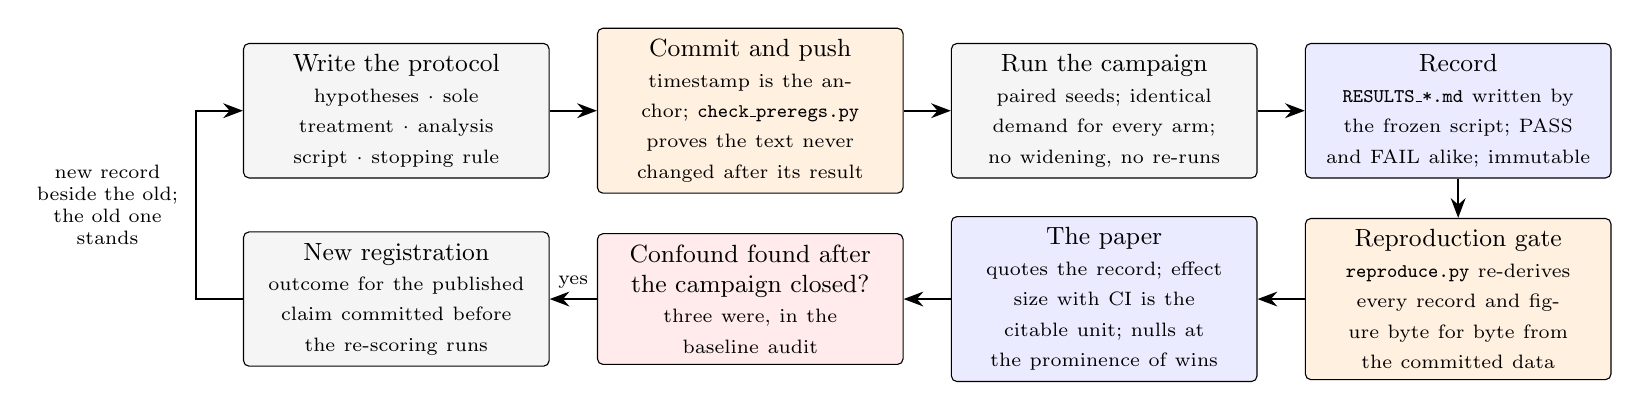
\begin{tikzpicture}[
  stage/.style={draw, rounded corners=2pt, align=center, font=\small,
               minimum height=11mm, text width=36mm, inner sep=4pt, fill=gray!8},
  gate/.style={stage, fill=orange!12},
  emit/.style={stage, fill=blue!8},
  bad/.style={stage, fill=red!8},
  arr/.style={-{Stealth[length=2.5mm]}, thick},
  node distance=5mm and 6mm
]
\node[stage] (prereg) {Write the protocol\\ \scriptsize hypotheses $\cdot$ sole treatment $\cdot$ analysis script $\cdot$ stopping rule};
\node[gate, right=of prereg] (push) {Commit and push\\ \scriptsize timestamp is the anchor; \texttt{check\_preregs.py} proves the text never changed after its result};
\node[stage, right=of push] (run) {Run the campaign\\ \scriptsize paired seeds; identical demand for every arm; no widening, no re-runs};
\node[emit, right=of run] (rec) {Record\\ \scriptsize \texttt{RESULTS\_*.md} written by the frozen script; PASS and FAIL alike; immutable};
\node[gate, below=of rec] (gate) {Reproduction gate\\ \scriptsize \texttt{reproduce.py} re-derives every record and figure byte for byte from the committed data};
\node[emit, left=of gate] (paper) {The paper\\ \scriptsize quotes the record; effect size with CI is the citable unit; nulls at the prominence of wins};
\node[bad, left=of paper] (conf) {Confound found after the campaign closed?\\ \scriptsize three were, in the baseline audit};
\node[stage, left=of conf] (re) {New registration\\ \scriptsize outcome for the published claim committed before the re-scoring runs};
\draw[arr] (prereg) -- (push);
\draw[arr] (push) -- (run);
\draw[arr] (run) -- (rec);
\draw[arr] (rec) -- (gate);
\draw[arr] (gate) -- (paper);
\draw[arr] (paper) -- (conf);
\draw[arr] (conf) -- node[above, font=\scriptsize]{yes} (re);
\draw[arr] (re.west) -- ++(-6mm,0) |- (prereg.west);
\node[font=\scriptsize, align=center, anchor=east] at ([xshift=-7mm]$(prereg.west)!0.5!(re.west)$) {new record\\ beside the old;\\ the old one\\ stands};
\end{tikzpicture}%
}
\caption{How a number reaches this paper. Orange boxes are gates a
machine checks; the red box is the one human judgement in the chain, and
its only permitted exit is a new registration. Forty-eight protocols took
this path; the withdrawn cost percentages of
Section~\ref{sec:eval-adjudication} are the loop's third pass.}
\label{fig:evidence-flow}
\end{figure}

\subsection{Baselines, tuned on our own objective}
\label{sec:method-baselines}

Five baselines carry the headline matrix: HPA-style reactive scaling,
KEDA-style event-driven scaling, a FIRM-style replica controller
\citep{firm2020}, GPTCache-style fixed semantic caching with LRU
\citep{gptcache2023}, and static provisioning. Later campaigns add a
VTC-style least-service-first replica divider \citep{vtc2024}, a
concurrency scaler in the Knative-KPA/AIBrix shape, a layered stack of
three locally tuned single-knob controllers, an offline-trained learned
joint controller, and iso-cost variants of the by-construction winners.
Every baseline is grid-search tuned on the composite objective this paper
is graded on, with the sweeps committed. Grids are bounded at a
vendor-sane envelope because $J$ improves monotonically toward
over-provisioning: an unbounded grid would tune every baseline into a cost
blow-out and flatter the joint controller. Iso-cost variants exist to
remove the ``it just spends less'' objection, and where their gate fails
it is reported as a failure. Two comparator corrections were added after
the audit of Section~\ref{sec:eval-adjudication}: \texttt{hpa\_fair} and
\texttt{keda\_fair}, which carry no eviction charge and a competently
pre-sized cache, and budget-carrying variants that apply the joint
controller's own per-tenant budget rule verbatim.
Table~\ref{tab:baselines} lists the grids and their winners; where a
vendor default exists, the tuned setting beats it on $J$, which is the
point of tuning.

\begin{table}[htbp]
\centering\tablefontsmall\setlength{\tabcolsep}{4pt}
\begin{tabularx}{\textwidth}{@{}>{\raggedright\arraybackslash}p{0.17\textwidth}>{\raggedright\arraybackslash}X>{\raggedright\arraybackslash}p{0.13\textwidth}rr@{}}
\toprule
\textbf{Baseline} & \textbf{Grid} & \textbf{Winner} & $J$ \textbf{best} & $J$ \textbf{default} \\
\midrule
HPA-style & target utilisation $\rho \in \{0.3, \dots, 0.8\}$ & $\rho = 0.3$ & 0.555 & 0.628 ($\rho = 0.8$) \\
KEDA-style & requests per replica $\in \{2, \dots, 16\}$ & 2.0 & 0.573 & --- \\
FIRM-style & learning rate $\times$ $\epsilon$ $\times$ SLO weight, 27 combinations & $0.1$, $0.1$, $4$ & 0.619 & 0.632 \\
GPTCache-style & target $\rho \in \{0.3, \dots, 0.8\}$, cache at maximum & $\rho = 0.3$ & 7.362 & 7.58 \\
VTC-replica & target $\rho \in \{0.3, \dots, 0.8\}$ & $\rho = 0.3$ & 0.555 & 0.628 \\
Concurrency (KPA shape) & target concurrency $\{0.5, \dots, 4.0\}$ $\times$ stable window $\{1, 3, 6\}$ intervals & $0.5$, $6$ & 0.543 & --- \\
Static & no knob: over-provisioned to the replica cap & --- & --- & --- \\
\bottomrule
\end{tabularx}
\caption{Baselines and their grid search on the composite objective
(\evfile{eval/baselines/TUNING.md}; tuning-slice $J$, lower is better).
The concurrency arm tunes to a stronger $J$ than tuned HPA or KEDA, so it
is not a straw man; KEDA and the concurrency scaler have no universal
vendor default. The winning stable window of six intervals is Knative's
60\,s.}
\label{tab:baselines}
\end{table}

\subsection{Substrates, never mixed}
\label{sec:method-substrates}

Three substrates carry the evidence, and no table in this paper mixes
them. The \emph{simulator} (Section~\ref{sec:system-model}) is the
decision-quality substrate. \emph{Real data replayed through the
simulator}: BurstGPT v2.0 demand \citep{burstgpt2024} (10,632,194 requests
over 335 days), Azure LLM inference 2024 demand \citep{azurellmtrace2024}
(44.1M requests, two production streams), and LMSYS-Chat-1M prompts
\citep{lmsyschat1m2024} embedded with a real MiniLM encoder
\citep{minilm2020,sbert2019}. And \emph{live clusters}: a kind cluster with
a real scheduler, real HPA and real load for the replica-only campaigns,
and a rented L40S host with a real inference tier behind the gateway for
the three-knob plane. Claims from the kind cluster are ordinal only---does
the simulator's ranking reproduce?---and absolutes are never compared
across substrates. Replay dollars are model-scale; the claim is always the
ranking. Samples from different replays are never pooled: the $n = 16$ and
$n = 96$ BurstGPT samples are separate experiments with separate
registrations.

\subsection{Statistics}
\label{sec:method-stats}

Runs are paired by seed: every system sees identical demand realisations,
including arrival jitter drawn once per window and shared across systems.
Significance is assessed with Wilcoxon or paired tests at the
pre-registered gate, Holm-corrected \citep{holm1979} where a hypothesis
spans several comparators. At hundreds of paired seeded simulator runs,
however, vanishing p-values measure the simulator's determinism rather
than the effect, so the citable unit throughout is the paired effect size
$\dz$ with a 95\% bootstrap confidence interval, following the reporting
discipline of Hoefler and Belli~\citep{hoefler2015benchmarking}: ratios are stated with
their absolute base, means are used for costs, tails get their own
statistic, and every varied factor is documented. All $n = 96$ confirmatory
intervals exclude zero, and the one violation trade that rides along
carries its own interval. P-values appear once, as gate outcomes, and are
never headlined below about $10^{-6}$. A weight-sensitivity sweep declared
before it ran perturbs the objective weights across 425 cells spanning
every campaign: the win direction never flips, and 416 of 425 cells keep
$p < 0.01$.

\subsection{Metrics}
\label{sec:method-metrics}

Cost in USD (replica-hours at \$0.048 per replica-hour; model-tier calls
at market ratios $1{:}10{:}100$), SLO violation rate, semantic-cache hit
rate, Jain's index over per-tenant SLO satisfaction, and the composite
\begin{equation}
\label{eq:J}
J = \mathrm{cost} + 2\cdot\mathrm{violation} + 0.5\cdot(1 - \mathrm{Jain}),
\end{equation}
normalised per tenant-step---the objective every baseline was tuned on.
Latency is reported at p95, not p99: the simulator's latency estimator is a
queueing approximation whose tail beyond p95 is not credible, and
pretending otherwise would be false precision. The live path measures
wall-clock latency and can report any percentile. After the adjudication
the saturating violation rate was joined by an unbounded severity metric,
mean SLO excess, on which some readings reverse; both are reported.

\subsection{The workload matrix}
\label{sec:method-matrix}

The headline matrix is a blocked factorial: 5 workload classes $\times$ 4
tenant-mix profiles $\times$ 3 cluster sizes $\times$ 6 systems $\times$ 5
repetitions, 1,800 runs, plus 500 ablation runs. Eight tenants per cluster
is the studied factor---composition, not population---and the planner's
tenant-count scaling is measured separately
(Section~\ref{sec:impl-scaling}). The overload cells of the third campaign
were sized by arithmetic on committed model constants---burst climbs that
exceed the shared $\pm 2$-replicas-per-interval actuation clamp---pinned
by unit tests rather than tuned by trial runs, with a same-envelope
control cell where the hypothesised advantage should not appear.

\subsection{Honest nulls}
\label{sec:method-nulls}

Negative and failed results are published with the prominence of wins, in
a dedicated ledger (\evfile{research/analysis/RESULTS\_MASTER.md}). The
ledger carries the two confirmatory SLO failures, the under-powered first
replay, the fairness-term null, the seasonal-forecasting non-transfer from
synthetic to real demand, the structurally impossible raw per-metric gate,
the cache hit-quality result, the live ordinal disagreement, the risk-knob
reversal, the withdrawn cost percentages, the published controller's loss
on the live plane and the damper's failure. Goalpost-moving is invisible
when it happens in private; here it happened in public, in git history,
where a reader can diff it.

\section{Evaluation}
\label{sec:eval}

We report every campaign in the order it was run, under the rules of
Section~\ref{sec:method}: wins, nulls and failures alike. Every number
traces to a committed, machine-generated record under
\evfile{research/analysis/} (\ref{app:traceability}); where a
sentence here and a record could disagree, the record wins. Each
subsection opens with the question it answers and closes with the answer.

\subsection{Does joint control win the objective it was built for?}
\label{sec:eval-scoreboard}

Yes, in every campaign that tested it, and the scoreboard in
Table~\ref{tab:scoreboard} states what survives in each of the six
contested segments after the adjudication of
Section~\ref{sec:eval-adjudication}.

\begingroup\tablefontsmall
\begin{longtable}{@{}>{\raggedright\arraybackslash}p{0.11\textwidth}>{\raggedright\arraybackslash}p{0.17\textwidth}>{\raggedright\arraybackslash}p{0.67\textwidth}@{}}
\caption{Verdicts across the six contested segments, as reconciled in
\evfile{RESULTS\_MASTER.md}. The cost row states the withdrawn history
beside the surviving claim, as every mention of it in this paper does.}
\label{tab:scoreboard}\\
\toprule
\textbf{Segment} & \textbf{Verdict} & \textbf{The citable claim} \\
\midrule
\endfirsthead
\caption[]{Verdicts across the six contested segments (continued).}\\
\toprule
\textbf{Segment} & \textbf{Verdict} & \textbf{The citable claim} \\
\midrule
\endhead
Cost & closed: feasibility, not performance (adjudicated) &
Against the originally tuned baselines the joint controller beat all five
on cost in the 1,800-run matrix and by $-70\%$ on replayed BurstGPT
demand. All of that is withdrawn as a like-for-like comparison: every
comparator carried an eviction charge and a pinned cache no \jcac{} arm
paid, and only \jcac{} was subject to the per-tenant budget filter. Against
fair comparators the matrix is cost-neutral versus \texttt{hpa\_fair}
($+0.8\%$, EP-H1a FAIL) with $-14.1\%$ versus \texttt{keda\_fair} surviving;
the BurstGPT figure shrinks to $-52.2\%$ and fails its own rank test;
against comparators carrying the budget rule BP-H1a/b FAIL on both traces.
What stands: the per-tenant budget is satisfiable only by a controller
holding the tier knob. \\
SLO & closed honestly: parity, bounded &
Violation parity with tuned HPA/KEDA at $-43$ to $-48\%$ cost; beats FIRM.
In overload, reactive scalers buy attainment at 3.2--3.4$\times$ the spend
(H1$'$ FAIL); the forecast mechanism is confirmed (H2$'$ PASS). On the
unbounded severity metric the synthetic advantage is understated by the
published metric and holds on Azure, but reverses on BurstGPT (TP-H3a/b
FAIL); lifting the budget cap removes 79\% of that gap as a typical-window
claim (BP-H2 PASS) whose tail still breaches the margin in 22\% of windows. \\
Fairness & won, two dedicated baselines &
Beats FIRM on Jain ($\dz = 1.0$); beats tuned VTC-replica on Jain itself
(0.9705 vs.\ 0.9599) at $-35\%$ cost. The controller's own $\gamma$ term
is a published null. \\
Forecasting & won, on real data &
Damped Holt $-26.9\%$ RMSE on real BurstGPT; the synthetic seasonal
prediction did not transfer and is published as such; on Azure LLM 2024
the mechanism boundary reproduces---the winner tracks measured periodicity. \\
Cache & closed, real-data headline &
29.6\% hits at cosine 0.85 and 48.8\% at 0.70 on real LMSYS-Chat-1M;
$+93\%$ over a 10\%-of-working-set fixed cache; \$0.296 saved per 1,000
queries; precision measured with its stochasticity ceiling. \\
Security & won, uncontested &
Timing side channel at AUC 0.88; per-tenant partitioning restores chance
at 24\% latency cost, dominating padding and TTL jitter; AUC 0.502 over
the wire. \\
\bottomrule
\end{longtable}
\endgroup

On the composite objective $J$ of Eq.~\eqref{eq:J}---the objective every
baseline was tuned on---the joint controller wins against every baseline
in every campaign that tested it: the 1,800-run matrix ($p \le
4.6{\times}10^{-25}$), the second matrix ($p \le 6.7{\times}10^{-25}$), the
overload matrix ($p \le 1.3{\times}10^{-11}$), the VTC slice ($p =
3.3{\times}10^{-19}$), the BurstGPT and Azure replays, the 2026-stack
concurrency arm ($p = 1.3{\times}10^{-44}$ at violation parity,
\evfile{RESULTS\_CONCURRENCY.md}), the 32-tenant slice ($p \le
2.2{\times}10^{-4}$, \evfile{RESULTS\_TENANT\_SCALE.md}), and an
offline-trained learned (RL) joint controller over the identical action
space ($p = 2.9{\times}10^{-28}$, $\dz = -0.708$, 95\% CI on the paired $J$
difference $[-0.437, -0.318]$; LR-H1/LR-H2 PASS,
\evfile{RESULTS\_LEARNED.md}). The learned policy is instructive rather
than merely beaten: it attains slightly lower violation than the MPC and
pays $2.61\times$ the spend for it, rediscovering the buy-headroom posture
of the reactive scalers instead of the cheap joint one. Finding the cheap
configuration, not meeting the SLO, is what the optimiser contributes.
Figure~\ref{fig:composite-objective} is the single-number ranking;
Figure~\ref{fig:pareto} shows that the joint controller is the only system
on the cost--violation frontier, and, read with no weights at all, it is
non-dominated in 48 of 60 cells---the most of any arm
(\evfile{RESULTS\_DOMINANCE.md}). These composite wins are scored against
the originally tuned baselines; the adjudication re-scores the cost and
SLO components separately, and Table~\ref{tab:scoreboard} already reflects
it.

\begin{figure}[htbp]
  \centering
  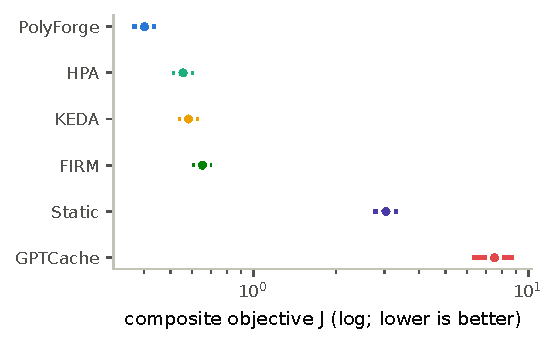
\includegraphics[width=0.8\textwidth]{fig12_composite_objective.pdf}
  \caption{The composite objective ($J = \mathrm{cost} +
  2\cdot\mathrm{violation} + 0.5\cdot(1-\mathrm{Jain})$, normalised per
  tenant-step): the single-number ranking every other figure decomposes.}
  \label{fig:composite-objective}
\end{figure}

\begin{figure}[htbp]
  \centering
  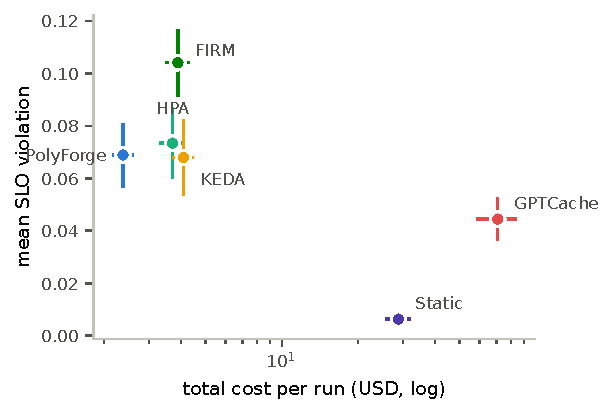
\includegraphics[width=0.8\textwidth]{fig03_pareto_cost_violation.pdf}
  \caption{The cost--violation plane (means $\pm$ 95\% CI over 300 cells
  per system): every baseline is dominated on at least one axis without
  winning the other.}
  \label{fig:pareto}
\end{figure}

\subsection{The headline matrix: where baselines break, and what each component is worth}
\label{sec:eval-matrix}

Does the taxonomy's control-implication column predict where single-knob
controllers fail, and does each of the controller's components carry
independent weight? Both, with one number that must not travel without its
caveat.

The blocked factorial of Section~\ref{sec:method-matrix}, all baselines
grid-tuned on $J$, gives the joint controller the composite win ($|\dz|$
0.66--1.44 against the five) and a violation rate held near the
over-provisioned floor at a fraction of that floor's cost. Where baselines
break is class-structured exactly as Table~\ref{tab:taxonomy} predicts:
replica-only controllers cannot fix agentic latency, because it needs the
tier knob (Figure~\ref{fig:violation-by-workload}). The single-trace view
shows the composed behaviour directly---within the first minute of an
agentic run the joint controller fills its replica budget and quadruples
the semantic cache while HPA chases each burst with the only knob it has.
Adaptive cache sizing doubles the fixed-cache baselines' hit share on
cacheable workloads and correctly declines to spend memory on uncacheable
ones. One pre-committed gate fails as measured and is reported: the
roadmap's raw per-metric gate (win every metric outright) is structurally
impossible against by-construction winners, since over-provisioned static
and cache-maxed GPTCache arms take the SLO and hit-rate columns at 12--30
times the joint controller's spend. The iso-cost variants exist for that
comparison (Section~\ref{sec:eval-slo}).

\begin{figure}[htbp]
  \centering
  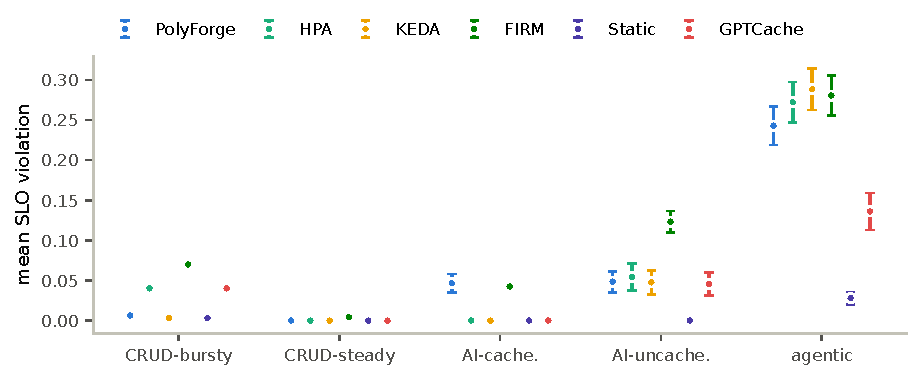
\includegraphics[width=0.88\textwidth]{fig07_violation_by_workload.pdf}
  \caption{SLO violation by workload class (mean $\pm$ 95\% CI): the
  taxonomy's control implications made measurable. Agentic latency is a
  tier-knob problem no replica-only controller solves.}
  \label{fig:violation-by-workload}
\end{figure}

\paragraph{Ablations (500 runs)} Removing joint control costs $+2884\%$
on the cost metric as published; removing cost-aware eviction $+35.7\%$;
removing the classifier $+2.1\%$ cost and $-45\%$ relative hit rate. Each
of the four components carries independent, statistically significant
weight (Figure~\ref{fig:ablations}). The first figure must not be cited
without its caveat. It rests on a defect in the layered/GPTCache
comparator: that arm ranks tiers by name and de-escalates only below
$0.3\times$ target, so on agentic traffic it escalates past the fastest
tier and sticks at the dearest one. A pre-registered re-scoring against a
competent layer-local tier rule (\evfile{PREREG\_LAYERED\_FIX.md}
$\to$ \evfile{RESULTS\_LAYERED\_FIX.md}) shrinks the ablation's cost delta
by $-86.4\%$ (LF-H1 PASS, $p = 1.2{\times}10^{-11}$); the composite win
over the corrected arm survives at the smaller margin (LF-H2 PASS, $p =
8.4{\times}10^{-16}$). The composition claim of this paper is the smaller,
surviving measurement, not the published multiple.

\begin{figure}[htbp]
  \centering
  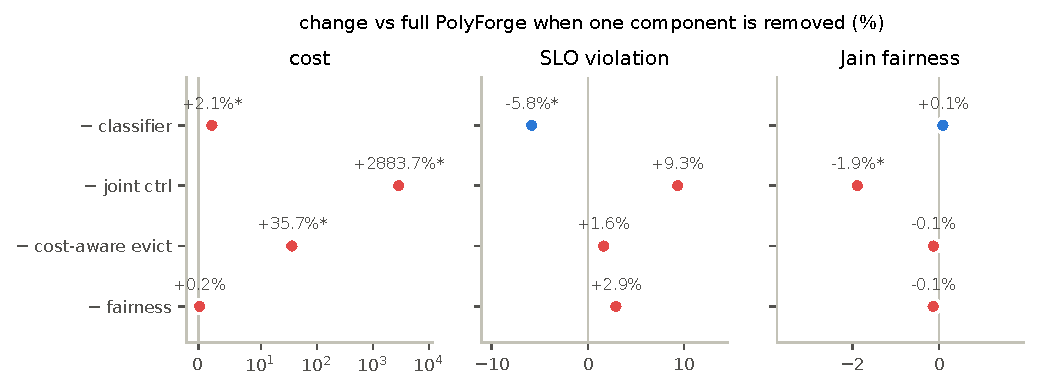
\includegraphics[width=0.85\textwidth]{fig08_ablation_deltas.pdf}
  \caption{Ablation deltas (red $=$ worse than the full controller; $* =
  p < 0.01$). The $-$joint bar is measured against the published layered
  comparator; against a competent tier rule it is 86\% smaller
  (Section~\ref{sec:eval-matrix}).}
  \label{fig:ablations}
\end{figure}

\subsection{SLO attainment: two failures, one mechanism, and a risk knob that moved the wrong way}
\label{sec:eval-slo}

Can the joint controller beat tuned reactive scalers on SLO attainment? We
tried twice under pre-registration, failed twice, and stopped by rule.
What holds is parity at much lower cost and a confirmed forecasting
mechanism.

\paragraph{Forecasters, realism, self-calibration} The in-loop forecast
ablation found headroom in the system's own default: the linear-trend
forecaster overreacts to bucket noise, and damped Holt smoothing beats it
by $-16.3\%$ SLO violation at equal cost ($p = 0.0027$;
Figure~\ref{fig:forecast-ablation}). Holt became the documented
recommended default; trend stays the code default so the committed
1,800-run headline remains bit-reproducible. Under reconfiguration realism
(replica start-up lag and half-warm caches, billed immediately), reactive
scalers pay for capacity that misses the burst it was bought for, while
the joint controller's hysteresis holds the frontier
(Figure~\ref{fig:realism-pareto}); self-calibration
(Proposition~\ref{prop:calibration}) earns $\dz = +0.46$ ($p = 0.029$),
concentrated on the bursty classes where trusting nominal capacity hurts
most.

\begin{figure}[htbp]
  \centering
  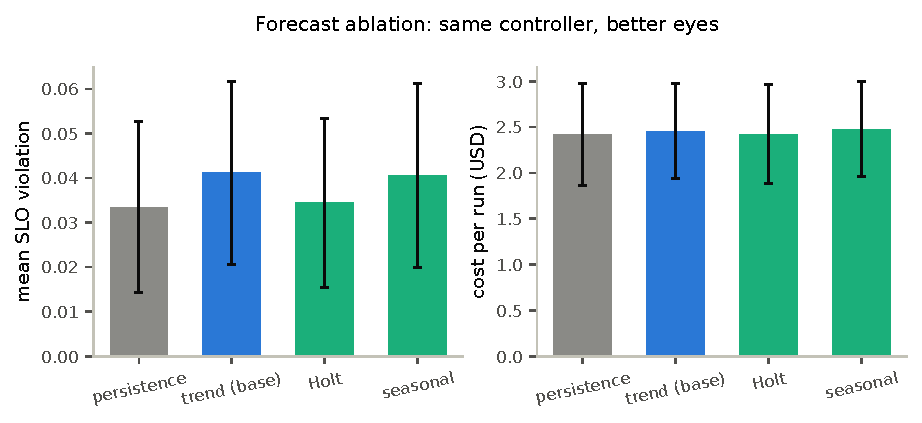
\includegraphics[width=0.8\textwidth]{fig13_forecast_ablation.pdf}
  \caption{Forecast ablation: damped Holt beats the trend default on
  violation at equal cost; online-seasonal detection helps only where a
  period exists.}
  \label{fig:forecast-ablation}
\end{figure}

\begin{figure}[htbp]
  \centering
  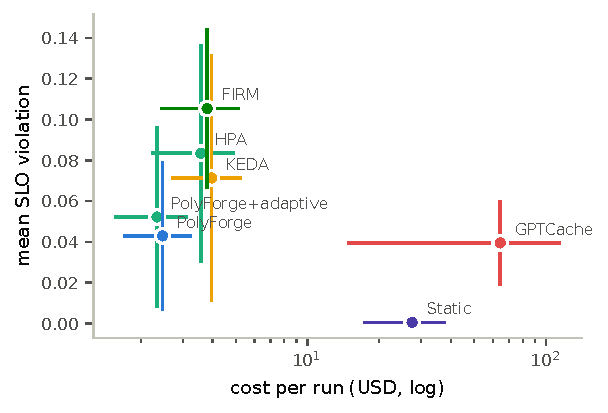
\includegraphics[width=0.8\textwidth]{fig14_realism_pareto.pdf}
  \caption{Under reconfiguration realism (replica start-up lag and cache
  warm-up, billed immediately): reactive scalers pay for capacity that
  misses the burst it was bought for, so their violations rise; the joint
  controller's hysteresis and the self-calibrating variant hold the
  frontier.}
  \label{fig:realism-pareto}
\end{figure}

\paragraph{The second matrix (\evfile{PREREG\_V2.md}, 2,100 runs)} The
protocol froze \texttt{jcac\_v2} (Holt plus adaptive capacity) and two
hypotheses. H1 failed: SLO violation is not significantly below tuned
HPA/KEDA. What holds is violation parity at $-43$ to $-48\%$ cost and a
clear win over FIRM ($p = 2{\times}10^{-19}$). H2 passed: no large-effect
self-regression, and cost improves $-11\%$ over the first controller
($p = 4{\times}10^{-36}$). The iso-cost gate reshapes the by-construction
winners: budget-matching turns static provisioning from a win-by-spending
into a three-of-five loss, and 36 of 60 cells are budget-infeasible for
the cache-max posture, which outspends the budget $36\times$. Per the
stopping rule, \texttt{jcac\_v2} was not re-tuned after the H1 failure.

\paragraph{The overload matrix (\evfile{PREREG\_V3.md}, 1,200 runs)}
The second matrix's demand shapes are smooth enough that reactive scalers
keep up; when everyone can react in time, everyone ties on violation and
cost is the only degree of freedom left. The third campaign therefore
constructed overload cells where demand climbs faster than the shared
actuation clamp, sized by arithmetic on committed constants
(Section~\ref{sec:method-matrix}), with \texttt{jcac\_seasonal} named in
advance as the sole treatment. H1$'$ failed, and the failure is
informative: tuned HPA and KEDA buy overload attainment with 3.2--3.4
times the joint controller's spend (seasonal is $-69$/$-71\%$ on cost at
$+0.05$/$+0.09$ violation), and only the joint controller honours the
cluster capacity cap at these amplitudes---a disclosed harness asymmetry,
strict against us. H2$'$ passed: seasonal forecasting reduces violations
against trend ($p = 6{\times}10^{-4}$) at no cost regression, so the
mechanism is real. In the declared-exploratory spike class, where reaction
is structurally impossible, the full predicted phenomenon appears:
seasonal beats HPA on violation ($p = 5{\times}10^{-5}$, $\dz = 0.57$) at
$-46\%$ cost. The pre-registered stopping rule closes confirmatory SLO
attempts: two attempts, two published failures, one confirmed mechanism.

\paragraph{The risk knob, twice} The published controller plans at the
expected demand, so realised demand lands above plan roughly half the
time---the mechanism behind the attainment-for-spend trade above. Two
pre-registered campaigns of 2,400 runs each scored a planning quantile as
an explicit risk knob. The first moved the controller the wrong way:
inflating projected demand also inflates projected tier spend, which trips
the per-tenant budget guardrail into its shed fallback, so a higher
quantile lowered spend and raised violation, monotonically---RQ-H1/RQ-H2
FAIL, published as a null (\evfile{RESULTS\_RISK.md}). The
one-changed-factor follow-up sizes capacity at the quantile but projects
cost and checks the budget at the point forecast: RB-H1 PASS at the
pre-declared $q = 0.90$, but the violation curve turns back up at $q =
0.95$, so the monotone frontier RB-H2 required is not claimed (RB-H2
FAIL), and strict domination of the reactive arms is not either (RB-H3
FAIL; \evfile{RESULTS\_RISK\_BUDGET.md}).

The answer to this subsection's question is no. The joint controller does
not beat tuned reactive scalers on attainment; it matches them at roughly
half the cost, the forecasting mechanism it relies on is real, and the
regime in which it wins on attainment---spikes that no reactive controller
can answer in time---is stated as exploratory.

\subsection{Real demand: two traces replayed}
\label{sec:eval-replay}

Does the ranking survive real demand? On the composite objective, yes, on
both traces. The cost percentages that came with it did not survive the
adjudication, and this subsection reports them as the history of the
claim.

Real BurstGPT v2.0 demand \citep{burstgpt2024}---10,632,194 requests over
335 days, normalised deterministically---was replayed through the
committed system model in six-hour windows, demand scale frozen pre-run,
arrival jitter drawn once per window and shared across systems. The first
sample ($n = 16$) failed its gate at $p < 0.01$, under-powered at $p
\approx 0.07$--$0.11$, though every point estimate reproduced the matrix
ranking; it stands as measured and is not the headline. The powered
second sample (\evfile{PREREG\_TRACE2.md}, $n = 96$ independent seeds,
about 94\% power) passed with disclosure: $J$ beats HPA, KEDA and FIRM
($\dz$ $-0.43$ to $-0.47$), cost was $-70\%$ against the baselines as tuned
(a figure withdrawn below), and the pre-registered disclosure was
honoured---a violation trade of $+0.07$ rides along, the same
attainment-for-spend trade quantified everywhere else. The second real
trace, Azure LLM inference 2024 \citep{azurellmtrace2024}, reproduced the
pattern at $-42\%$ per window against the same comparators as tuned
(\evfile{RESULTS\_TRACE\_AZURE.md}), a figure withdrawn on the same grounds.

Neither cost figure is this paper's claim. Both were re-scored after the
campaigns closed against comparators corrected for the confounds an audit
found (Section~\ref{sec:eval-adjudication}): the BurstGPT advantage
shrinks from $-70.4\%$ to $-52.2\%$ at eviction parity and fails its own
pre-registered rank test; Azure shrinks from $-42.5\%$ to a real but small
$-7.1\%$; and against comparators carrying the joint controller's own
budget rule both fail. The replay records stand exactly as committed, as
the ground rules require; the numbers in them are reported here as
history, not as results.

\subsection{Adjudication: the cost and SLO claims under fair comparators}
\label{sec:eval-adjudication}

What survives when the baselines are corrected for every asymmetry an
audit could find? A feasibility statement about the budget, a bounded SLO
reading, and nothing of the comparative cost percentages.

After the campaigns above had closed, an audit of the baseline
implementations found three asymmetries between the joint controller and
every comparator it had been scored against. Each was addressed by a
pre-registered re-scoring against a corrected comparator, with the outcome
for the published claim committed before the run. None of the original
records was edited; every re-scoring is a new record.

\paragraph{Eviction parity} (\evfile{PREREG\_EVICTION\_PARITY.md} $\to$
\evfile{RESULTS\_EVICTION\_PARITY.md}.) Every reactive comparator
carried a $1.4581\times$ LRU inference charge that no \jcac{} arm paid, and
was pinned at a 128\,MB cache it could not move. Against \texttt{hpa\_fair}
and \texttt{keda\_fair}---no charge, competently pre-sized at 512\,MB---the
1,800-run matrix is cost-neutral against \texttt{hpa\_fair} ($+0.8\%$,
EP-H1a FAIL) while $-14.1\%$ against \texttt{keda\_fair} survives ($p =
3.8{\times}10^{-16}$). The same record introduces the unbounded severity
metric, mean SLO excess, on which the synthetic SLO advantage is understated
by the published rate: 0.2143 against 0.4288 for \texttt{hpa\_fair}, roughly
half.

\paragraph{Trace parity} (\evfile{PREREG\_TRACE\_PARITY.md} $\to$
\evfile{RESULTS\_TRACE\_PARITY.md}.) The two real-demand headlines
re-scored against the fair comparators. Azure: $-7.1\%$, real and
pervasive (TP-H1a/b PASS, $p \le 9.5{\times}10^{-5}$, 69.4\% of windows
favour the joint controller), with the SLO pattern holding within margin
(TP-H3a/b PASS). BurstGPT: $-52.2\%$ on the mean but TP-H1a FAIL ($p =
0.0133$ against a Holm threshold of $0.01250$)---the advantage is
concentrated in a minority of windows, and the joint controller is the
dearer system in 57.3\% of six-hour windows. On severity BurstGPT
reverses: the joint controller's mean excess is 0.5134 against 0.0088 for
\texttt{hpa\_fair}, $58\times$ worse, breaching the 0.05 non-inferiority
margin in 41.7\% of windows, with AI requests shed on 9.3\% of
tenant-steps against none for any reactive arm (TP-H3a/b FAIL). The ``half
the overshoot'' reading is therefore synthetic-and-Azure only, and it is
never stated in this paper without the BurstGPT reversal beside it.

\paragraph{Budget parity} (\evfile{PREREG\_BUDGET\_PARITY.md} $\to$
\evfile{RESULTS\_BUDGET\_PARITY.md}.) The fair comparators removed the
eviction and cache-posture confounds but not a third: only the joint
controller was ever subject to the per-tenant budget filter---it rejects
over-budget candidates before its objective is evaluated, and no baseline
planner has a cost term at all. Scored against comparators carrying the
controller's own budget rule verbatim, BP-H1a/b FAIL on both traces
(Azure $-3.3\%$/$-1.3\%$, $p = 0.379$/$0.91$; BurstGPT
$-50.2\%$/$-49.8\%$, $p = 0.112$/$0.191$---again a minority-of-windows mean
that does not survive the rank gate). Per the response committed before
the run, the like-for-like cost claim is withdrawn, not restated.
Amendment~1, disclosed before scoring, explains why no better comparator
can rescue it: at the per-tenant cap, tier spend dominates infrastructure
spend by three orders of magnitude, and capping a replica-only arm moves
its infrastructure spend by $-45.7\%$/$-57.4\%$ and its tier spend by
exactly 0.00\% on both traces. No budget-respecting comparator exists in
the replica-only class. That is the claim that survives, and it is sharper
than a percentage: the per-tenant budget is a promise only a controller
holding the tier knob can keep. On the SLO side, lifting the joint
controller's budget cap removes 79\% of the BurstGPT severity gap (BP-H3)
and BP-H2a/b PASS on both traces---bounded, on BurstGPT, to a
typical-window claim: the median difference is exactly 0.0000 and 51\% of
windows are no worse, but the mean difference ($+0.1037$) exceeds the
margin the rank test passed, 22\% of windows breach it, and the worst
breaches it $59\times$. A descriptive follow-up, not pre-registered and
quotable only as characterisation, finds that the cost win and the SLO
penalty are the same windows.

\paragraph{Robustness of what remains} The sweep-order confound the same
audit raised is real but immaterial: permuting the tenant sweep moves Jain
by at most 0.0001 against a pre-registered 0.01 threshold (OP-H1 fails
strictly as a sensitivity bound; OP-H3 PASS on cost;
\evfile{RESULTS\_ORDER\_PERMUTATION.md}), and the sweep seed is now an
explicit parameter. The controller also survives being wrong about its own
plant: with each plant constant perturbed $\pm 25\%$ one at a time, the
cost win over \texttt{keda\_fair} survives on every constant (MM-H1 PASS)
and severity stays within the inherited margin (MM-H2 PASS;
\evfile{RESULTS\_MODEL\_MISMATCH.md})---mismatch-robust within that band,
one constant at a time, and quoted with that scope.

\subsection{Forecasting on real traces: a prediction fails to transfer, a boundary reproduces}
\label{sec:eval-forecast}

Does the forecaster that wins on synthetic demand win on real demand? No;
and the reason it does not is the result.

The synthetic stand-in (a textbook diurnal with autocorrelation 0.85 at
24\,h) predicted that seasonal forecasting would dominate, at $-44.8\%$
RMSE. On real BurstGPT the periodicity is weak (best autocorrelation $\le
0.49$ at 8\,h) and the prediction does not transfer: seasonal never beats
trend; damped Holt wins the first segment ($-26.9\%$ RMSE), persistence
wins the second ($-16.6\%$), and trend is the worst choice on real data.
The recommendation followed the data. The Azure LLM 2024 trace---44.1M
requests, two production streams---reproduces the mechanism boundary
through the identical frozen decomposition: seasonal wins exactly on the
stream with a genuine daily cycle (the code stream, $-15.6\%$ RMSE at
autocorrelation 0.57, lag 24), loses on the weakly periodic conversation
stream ($+48.5\%$; persistence wins), and pooling the streams destroys
forecastability (seasonal $+104\%$). Across three real streams no fixed
forecaster dominates, and the winner tracks measured periodicity. The
same traces split by model and log type into 19 sub-streams reproduce the
boundary with zero counter-examples, every periodic sub-stream shows the
seasonal win, and three different forecasters win across sub-streams
(PT-H1/H2/H3; \evfile{PSEUDO\_TENANT.md})---exactly what a pluggable
per-tenant forecasting layer exists to exploit. That is the external
support for the per-stream design, and it is the scoped version of the
H2$'$ result.

\subsection{The semantic cache on real prompts}
\label{sec:eval-cache}

What does the cache deliver on real prompts, and how often is a hit the
wrong answer? A 29.6\% hit rate at cosine 0.85, dollar-weighted; and a
precision that a stochasticity ceiling, not the retrieval, bounds.

On LMSYS-Chat-1M \citep{lmsyschat1m2024} (a seeded reservoir sample of
200,000 from 2,015,645 user turns; MiniLM embeddings; block-wise exact
nearest neighbour verified bit-identical against the dense computation;
feasibility amendments committed before the gated download), adaptive
sizing reaches 29.6\% hits at cosine 0.85 and 48.8\% at 0.70. InstCache's
51.34\% on the same dataset \citep{instcache2024} is a different mechanism
(pre-populated predicted instructions) and is placed beside, never
head-to-head. Against a non-strawman fixed baseline---a cache at 10\% of
the inserted working set---adaptive sizing is $+93\%$ (29.6\% against
15.3\%); in the matrix it is $+83\%$ over fixed (0.106 against 0.058). The
saving is \$0.296 per 1,000 queries at mid-tier pricing, a figure
cache-only papers cannot produce because it needs the tenant-tier
accounting. The empirical capacity curve fits $h_{\max} = 0.285$ with
half-saturation at about 6,569 entries (roughly 19\,MB); the simulator's
assumed curve was optimistic, the fit is documented beside it, and the
committed constants are unchanged for bit-reproducibility.

\paragraph{Hit quality} A hit that serves the wrong answer is not a
saving, so precision was measured under a frozen protocol
(\evfile{CACHE\_PRECISION.md}): the probability, given a hit, that the
served response agrees with the actually received response at agreement
threshold 0.70, with same-model and first-turn strata declared pre-run. At
$\tau = 0.85$ precision is 0.313 overall, 0.443 same-model and 0.353
first-turn; 165.5 incorrect hits per 1,000 queries are reported beside the
savings. The built-in calibration bounds the reading: near-duplicate
prompts at $\tau \ge 0.95$ agree only 33.8\% of the time, because 25
models and sampling temperature dominate the absolute level. The citable
claims are therefore relative: precision rises monotonically as $\tau$
tightens (0.249 to 0.338) while hit rate falls, and same-model precision
is about twice cross-model (0.443 against 0.223), so a deployment caching
one model's responses sits in the most favourable stratum. A later
pre-registered probe located the ceiling itself
(\evfile{RESULTS\_CACHE\_CEILING.md}, C1 PASS): with perfect retrieval---oracle
same-model duplicate pairs---precision reaches only 0.4898, so removing
every retrieval error recovers $+0.047$. The binding constraint on hit
quality is response stochasticity, not the embedder or the threshold.

\subsection{Fairness: two dedicated baselines beaten, the controller's own term nulled}
\label{sec:eval-fairness}

Is the joint controller fairer than controllers built for fairness, at
the altitude it works at? Yes, on Jain's index against both, and the win
is an emergent property of joint allocation rather than of the designed
fairness term.

Against FIRM-style control the joint controller wins Jain's index 0.9689
against 0.9294 in the headline matrix ($\dz = 1.0$, $p =
4.5{\times}10^{-47}$), replicated in the second matrix (0.9672 against
0.929, $\dz = 0.95$). Against the tuned VTC-style replica divider
\citep{vtc2024} under interference injection (\evfile{PREREG\_VTC.md}, 200
runs): HV1 PASS---the dedicated fair divider loses the composite objective
($\dz = -1.12$, $p = 3{\times}10^{-19}$)---and HV2 PASS: it does not buy a
fairness win either, since the joint controller is more fair on Jain
itself (0.9705 against 0.9599, $p = 1.5{\times}10^{-6}$) at $-35\%$ cost and
$-36\%$ worst-tenant p95. This is capacity-allocation fairness at the
control plane, not token-level service fairness
(Section~\ref{sec:threats}).

The controller's own $\gamma$ term is a published null: under injected
noisy-neighbour interference the $\gamma$-ablation shows no significant
contribution, even in the whale-only subgroup where the injection fires
(\evfile{FAIRNESS\_V2.md}). The term stays in the system as a configurable
weight and is dropped from the claims. Fairness is claimed as a measured
outcome, not as a mechanism.

\subsection{Security: a timing side channel and its defence frontier}
\label{sec:eval-security}

Can a shared semantic cache leak which tenant asked what, and what does
closing the leak cost? Yes, from response time alone, at AUC 0.88; and
per-tenant partitioning closes it at 24\% latency cost while every other
defence stays leaky or discards most of the cache.

A shared semantic cache leaks prompt membership across tenants: an
attacker distinguishing whether a victim tenant inserted a prompt reaches
AUC 0.88 from timing alone (compare the API-layer audit of
Gu et al.~\citep{promptcacheaudit2025}). Per-tenant partitioning returns the attacker
to chance (AUC 0.50) at 24\% latency cost while keeping 76\% of hits,
strictly dominating response-time padding (never below AUC 0.73 at any
cost) and TTL jitter (chance only at about 90\% hit loss) on the
leakage-versus-benefit frontier (Figure~\ref{fig:defense-frontier}). This
measurement is what made the gateway's cache per-tenant by default. The
frontier was then confirmed over the wire, against the real gateway process
rather than the simulator (\evfile{RESULTS\_WIRE\_ATTACK.md}): with the
per-tenant posture the membership attack lands at AUC 0.502 (95\% CI
$[0.384, 0.612]$)---chance, on the real HTTP and cache path---WA-H1 PASS,
while the deliberately shared posture leaks perfectly on loopback (AUC
1.000, all 50 victim secrets recovered; WA-H2, reported as measured).

\begin{figure}[htbp]
  \centering
  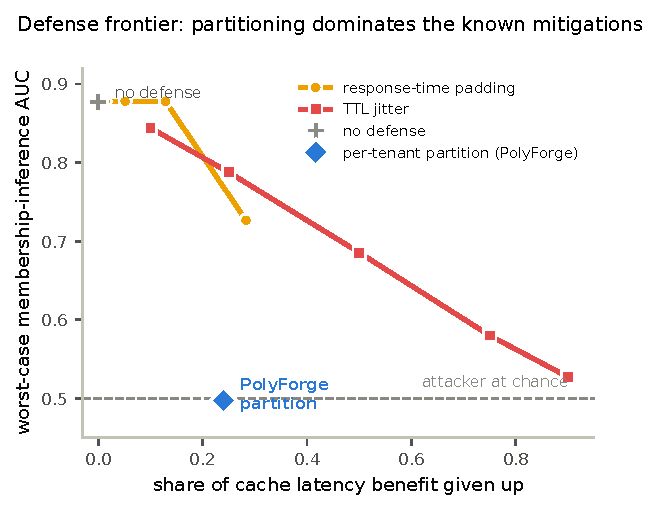
\includegraphics[width=0.8\textwidth]{fig17_defense_frontier.pdf}
  \caption{Defence frontier: worst-case membership-inference AUC against
  the share of the cache's latency benefit given up, same attack for every
  defence. Per-tenant partitioning reaches chance at a fraction of the
  cost padding and TTL jitter require, and dominates the frontier rather
  than joining it.}
  \label{fig:defense-frontier}
\end{figure}

\subsection{Live evidence}
\label{sec:eval-live}

Does any of this survive a real scheduler, a real autoscaler and a real
inference tier? In the order the campaigns ran: the replica-only ordinal
check recorded a disagreement; a 24-hour soak was valid with two of four
hypotheses failed; a real trace drove the real cluster and the cost
ordering matched; and on the three-knob live plane the published
controller lost to its own ablation, a corrected controller then beat
every arm at equal fairness, and the obvious damper failed. Absolutes are
never compared across substrates anywhere in this subsection.

\paragraph{The ordinal check, and its disagreement} The kind-cluster
experiment asks only whether the simulator's \jcac{}-versus-HPA ranking
reproduces under a real scheduler, real HPA and real load. The joint
controller's first live execution passed its smoke on the first attempt,
with the actuation gate passed before load, and the mirrored slice
completed with 12 of 12 valid runs (two arms $\times$ two cells $\times$
three repetitions), analysed by a protocol frozen before any live number
existed (\evfile{PHASE7\_ORDINAL.md}). As measured, the primary reading is
a disagreement: the $J$ winner flips in both cells
(Table~\ref{tab:ordinal}). The descriptive detail the protocol permits is
that live, the two arms land at parity on every metric---$J$ separations
of 0.002 with overlapping ranges, zero violations for both arms in both
cells---while the simulator separates them decisively. Two mechanisms
account for it. In the cacheable cell the simulator's win flows through the
cache economy, and the live cache knob is inert by construction on this
substrate, as the caption frozen before the run discloses. In the bursty
CRUD cell the simulator's HPA concedes 0.0417 violation under the burst
while real HPA at this amplitude, under the small-cluster capacity cap,
never violates: the simulator overestimates reactive-scaler lateness in
this cell, a model datum recorded as such, in a direction that favoured
the joint controller in-simulator. The verdict is DISAGREE and it stands.
What the campaign establishes is that the full loop runs live---features
to planner to operator actuation, mechanically gated---with capacity
parity held and neither arm degrading; what it does not establish is
reproduction of the simulator's ranking on the replica-only projection at
this amplitude.

\begin{table}[htbp]
\centering\tablefont
\begin{tabular}{@{}llrrr@{}}
\toprule
\textbf{Cell / substrate} & \textbf{arm} & $J$ \textbf{mean [min..max]} & \textbf{cost \$} & \textbf{violation} \\
\midrule
ai\_cacheable, sim  & jcac & 0.596 [0.593..0.601] & 5.66 & 0.0006 \\
                    & hpa  & 0.921 [0.917..0.924] & 8.77 & 0.0000 \\
ai\_cacheable, live & jcac & 0.739 [0.738..0.739] & 7.03 & 0.0000 \\
                    & hpa  & 0.737 [0.735..0.740] & 7.02 & 0.0000 \\
\addlinespace
crud\_bursty, sim   & jcac & 0.040 [0.040..0.040] & 0.38 & 0.0000 \\
                    & hpa  & 0.136 [0.136..0.136] & 0.30 & 0.0417 \\
crud\_bursty, live  & jcac & 0.027 [0.027..0.027] & 0.26 & 0.0000 \\
                    & hpa  & 0.025 [0.023..0.027] & 0.24 & 0.0000 \\
\bottomrule
\end{tabular}
\caption{Live ordinal check on a kind cluster: does the simulator's
jcac-versus-HPA ranking reproduce under a real scheduler, real HPA and real
load? Absolutes are not comparable across substrates and are not compared.
The live data plane burns fixed CPU per request kind, so the cache and tier
knobs are inert here; this table validates the replica-control projection
of the joint controller only. The caption's disclosure was frozen verbatim
before the run.}
\label{tab:ordinal}
\end{table}

\paragraph{Endurance, placement, and a real trace live} The live CRUD
plane was held under load for a full day (\evfile{PREREG\_LIVE\_SOAK\_V8.md}
$\to$ \evfile{RESULTS\_LIVE\_SOAK\_V8.md}): 24\,h\,00\,m\,11\,s, 25,806,353
requests at 298.6 per second, 0.0012\% failed, zero dropped iterations and
zero pod restarts---SK-H4 PASS on the absolute validity rule that had ended
four earlier attempts and was never relaxed, and SK-H2 (audit continuity)
PASS. The result is split and both halves are the finding: SK-H1 FAIL
(recovery within a 20\% band after fault injection fails on one of eight
injections) and SK-H3 FAIL (hourly CRUD p95 $\le 8.0072$\,ms exceeded in
six of 25 buckets). The earlier attempts are published as INVALID or VOID
with their causes traced---a port-forward that pinned all load to one pod
of sixteen, then host power-source flapping that opened 48--51\,s
scheduling gaps---none of them the controller. A descriptive follow-up
shows the frozen SK-H1 rule scores peak-against-trough on a four-minute
latency oscillation present before, during and after the failing
injection, so it cannot tell that fault from a quiet minute; SK-H1 stays
failed as scored. On a four-node cluster the load actually spread: three
nodes carried work and the busiest held 0.3815 of it, below the frozen
0.90 pinning threshold (MN-H1 PASS; \evfile{RESULTS\_MULTINODE.md}). And
window 0 of the BurstGPT trace drove the real cluster
(\evfile{RESULTS\_TRACE\_LIVE.md}): the live cost ordering matches the
simulator's (TL-H1 PASS); on violation both substrates rank the arms equal
(TL-H2 vacuous); the substrate delivered the registered demand within the
quantisation of a one-minute time unit (TL-H3 PASS).

\paragraph{The three-knob live plane: B1, B1$'$, B1$''$} That substrate
was then rented: one L40S host (8 vCPU, 62\,GiB) with a real inference tier
behind the gateway, so that all three knobs are live and every arm is
scored on the same four cells (\texttt{ai\_cacheable}, \texttt{tier\_mixed},
\texttt{crud\_bursty}, \texttt{joint\_stress}) under protocols frozen before
any number existed.

\emph{B1} (\evfile{PREREG\_WAVE4\_LIVE\_PLANE.md} $\to$
\evfile{RESULTS\_WAVE4\_LIVE\_PLANE.md}): the published joint controller
lost its primary reading. In \texttt{joint\_stress} it cost \$0.3651 against
\$0.2960 for the cheapest single-knob arm (tier-only, $+23.3\%$ for the
joint controller) at equal fairness---WL-H1 FAIL---with the knob-liveness
gate WL-H2 passing in all sixteen windows. Losing to one's own ablation is
a defect in the optimisation, not a fact about jointness. The defect was
found in two parts---an open-loop plant model that was pessimistic by three
orders of magnitude about the live tier's latency, and a hysteresis ratchet
that let a pessimistic plan lock in---and corrected as an opt-in arm,
\texttt{jcac-calibrated}, under a new frozen protocol.

\emph{B1$'$} (\evfile{PREREG\_WAVE4\_CALIBRATED.md} $\to$
\evfile{RESULTS\_WAVE4\_CALIBRATED.md}; Table~\ref{tab:b1prime},
Figure~\ref{fig:calibrated-plane}): the corrected controller beats every one
of the four comparators on cost at iso-fairness in \texttt{joint\_stress},
each with a paired-bootstrap interval excluding zero---WL-H1$'$ PASS
(\$0.2650, Jain 1.000)---and the per-cell ablation dominance WL-H4 passes
in all four cells. The paired bootstrap assumes independent buckets and the
deltas are autocorrelated (lag-1 autocorrelation up to $+0.81$); a
moving-block bootstrap at block lengths 5 and 10 leaves every interval
below zero (\evfile{SENSITIVITY\_WAVE4\_CALIBRATED.md}). The record also
prints, beside the win, that the corrected controller oscillates its
replica count (8--24 replicas in \texttt{tier\_mixed};
\evfile{CHURN\_WAVE4\_CALIBRATED.md}). With its plant fitted to this live
evidence under a rule frozen beforehand, the simulator's cost winner then
matches the live one in three of four cells, against one of four for the
published plant (WL-H3$'$ PASS; \evfile{RESULTS\_WAVE4\_SIM\_TRANSFER.md}).
The ordinal disagreement of the earlier campaigns was a plant-calibration
gap, not a ranking the simulator cannot express.

\begin{table}[htbp]
\centering\tablefontsmall\setlength{\tabcolsep}{4pt}
\begin{tabular}{@{}lrrrrl@{}}
\toprule
\textbf{versus arm} & \textbf{arm cost \$} & $\Delta$\textbf{cost \$} & $\Delta\%$ & \textbf{95\% CI, $\Delta$/bucket} & \textbf{beats} \\
\midrule
\polyforge{} (published) & 0.3332  & $-0.0682$  & $-20.5\%$ & $[-0.0030, -0.0016]$ & yes \\
replica-only             & 26.7047 & $-26.4397$ & $-99.0\%$ & $[-1.0781, -0.6507]$ & yes \\
cache-only               & 1.5120  & $-1.2470$  & $-82.5\%$ & $[-0.0451, -0.0347]$ & yes \\
tier-only                & 0.3220  & $-0.0570$  & $-17.7\%$ & $[-0.0027, -0.0009]$ & yes \\
\bottomrule
\end{tabular}
\caption{B1$'$, the pre-registered primary reading (WL-H1$'$): the
calibrated joint controller (\$0.2650, Jain 1.000) against every other arm
in \texttt{joint\_stress} on one L40S host. ``Beats'' requires lower mean
cost, Jain within 0.01, and a 95\% paired-bootstrap interval on the
per-10-s-bucket cost delta (calibrated minus arm, paired by position, reps
pooled, 10,000 resamples, seed 20260915) entirely below zero. Every arm's
Jain is within 0.004 of the calibrated arm's.}
\label{tab:b1prime}
\end{table}

\begin{figure}[htbp]
  \centering
  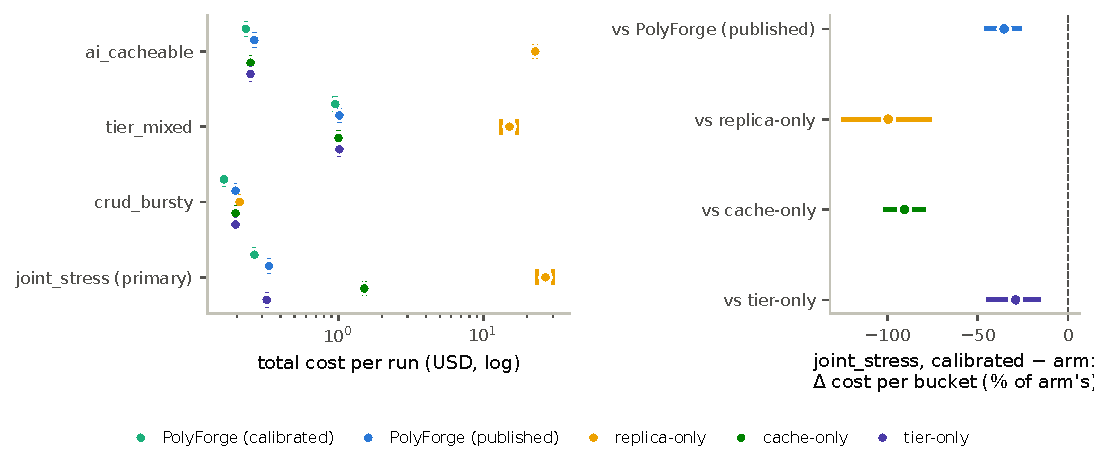
\includegraphics[width=\textwidth]{fig20_calibrated_plane.pdf}
  \caption{B1$'$ on one L40S host, five arms $\times$ four cells $\times$
  two reps. Left: total cost per run at iso-fairness (every arm's Jain index
  is within 0.01 of the calibrated arm's in every cell shown; the record
  lists the exceptions); dots are the mean of two reps, ticks the reps.
  Right: the pre-registered primary reading---in \texttt{joint\_stress} the
  calibrated joint controller's cost per 10-s bucket minus each arm's,
  paired by position within the load window, as a percentage of that arm's
  mean bucket cost, with the 95\% paired-bootstrap CI; a CI entirely left of
  zero is a win. Won against the published controller, replica-only,
  cache-only and tier-only.}
  \label{fig:calibrated-plane}
\end{figure}

\emph{B1$''$} (\evfile{PREREG\_WAVE4\_DWELL.md} $\to$
\evfile{RESULTS\_WAVE4\_DWELL.md}; Figure~\ref{fig:dwell-plane}) tested the
obvious damper, a three-cycle replica dwell, against the arm it damps. It
caps the largest single jump but does not halve the churn (WL-H6 FAIL:
20.0 against 22.0 changes per window in \texttt{joint\_stress}, 12.0
against 8.0 in \texttt{ai\_cacheable}), and its cost is not shown
non-inferior to the calibrated arm's (WL-H7 FAIL: $+2.0\%$, interval
$[-0.0006, +0.0012]$ per bucket against a bound of $+0.0002$; it still
beats tier-only by $-31.4\%$). The oscillation is a slow swing, not
chatter, so the next damper must act on the plant-estimate feedback rather
than on move reversals. It has not been built and is not pre-registered.

\begin{figure}[htbp]
  \centering
  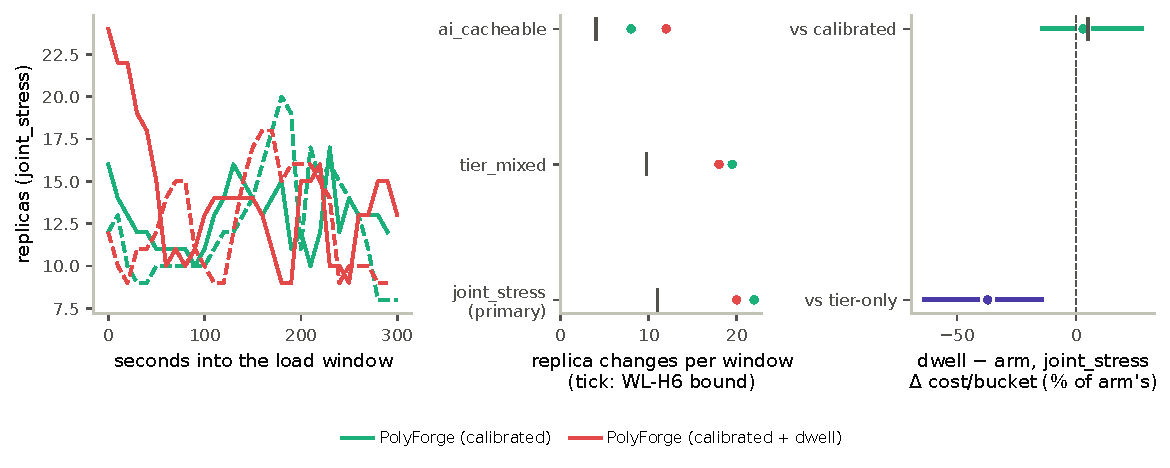
\includegraphics[width=\textwidth]{fig21_dwell_plane.pdf}
  \caption{B1$''$ on one L40S host, three arms $\times$ four cells $\times$
  two reps, scored from the load window only. Left: the replica count every
  10\,s through the \texttt{joint\_stress} window for the dwell-damped
  controller and the calibrated controller it damps (solid rep 0, dashed
  rep 1)---the oscillation is a slow swing, which a dwell on reversals
  cannot remove. Middle: WL-H6---replica-count changes per window in the
  three AI cells; the tick is the pre-registered bound, half the calibrated
  arm's changes, and the dwell arm must sit left of it: FAIL. Right:
  WL-H7---the dwell arm's cost per 10-s bucket minus each arm's, with the
  95\% paired-bootstrap CI; the tick on the calibrated row is the $+5\%$
  non-inferiority bound. Non-inferior to the calibrated arm: not shown;
  beats tier-only: yes.}
  \label{fig:dwell-plane}
\end{figure}

The answer for the live substrate is therefore layered. The replica-only
projection did not reproduce the simulator's ranking; the three-knob plane
did, once the plant was calibrated, and the corrected controller's cost win
at iso-fairness is the one live result in this paper on which every knob
was live and every arm was scored on the same cells. It comes with an
oscillation the first damper did not fix.

\subsection{Which number to cite}
\label{sec:eval-summary}

Table~\ref{tab:which-number} is the disambiguation a reader needs to quote
this paper correctly. The conservative column is the claim; the right-hand
column is what a hurried reading might take away and should not.

\begingroup\tablefontsmall
\begin{longtable}{@{}>{\raggedright\arraybackslash}p{0.16\textwidth}>{\raggedright\arraybackslash}p{0.42\textwidth}>{\raggedright\arraybackslash}p{0.37\textwidth}@{}}
\caption{Disambiguation table, from \evfile{RESULTS\_MASTER.md}. The cost
rows quote withdrawn figures only to name them as withdrawn.}
\label{tab:which-number}\\
\toprule
\textbf{Claim} & \textbf{Cite} & \textbf{Not} \\
\midrule
\endfirsthead
\caption[]{Disambiguation table (continued).}\\
\toprule
\textbf{Claim} & \textbf{Cite} & \textbf{Not} \\
\midrule
\endhead
Cost, the claim & the per-tenant budget is satisfiable only by a
controller holding the tier knob; no replica-only reactive controller can
meet it (tier spend moves 0.00\% under any replica cap) & any comparative
percentage against the originally tuned baselines \\
Cost, real demand & Azure $-7.1\%$ at eviction parity (TP-H1a/b PASS);
BurstGPT: no rank-test-surviving advantage & the withdrawn $-70\%$ and
$-42\%$; $-52.2\%$ (mean only, fails its rank test) \\
Cost, synthetic matrix & $-14.1\%$ vs.\ \texttt{keda\_fair}; cost-neutral
vs.\ \texttt{hpa\_fair} & the matrix percentages vs.\ HPA/KEDA/FIRM as
tuned; any mixing with replay numbers \\
Composition (ablation) & removing joint control worsens cost at the margin
that survives a competent tier rule (LF-H1: delta $-86.4\%$ vs.\ published)
& $+2884\%$ without its comparator caveat \\
Forecasting & Holt $-26.9\%$ RMSE on real BurstGPT; the winner tracks
measured periodicity across three traces & seasonal $-44.8\%$ (synthetic;
did not transfer); ``Holt is best'' \\
SLO & parity at $-43$ to $-48\%$ cost; mechanism $p = 6{\times}10^{-4}$;
severity half of \texttt{hpa\_fair}'s on synthetic and Azure with the
BurstGPT reversal ($58\times$) beside it & ``beats HPA/KEDA on violation'';
``half the overshoot'' alone \\
Fairness & Jain 0.9705 vs.\ VTC 0.9599; FIRM $\dz = 1.0$ & the
$\gamma$-ablation (published null) \\
Cache & 29.6\% at 0.85 on real LMSYS, $+93\%$ vs.\ 10\%-fixed;
precision-vs-$\tau$ shape and strata & synthetic saturation; ``69\% of hits
are wrong'' (ignores the ceiling) \\
Security & AUC 0.88 $\to$ 0.50 at 24\% latency, 76\% hits kept; 0.502 over
the wire & --- \\
Live, replica-only & loop verified end to end; ordinal check DISAGREE; 24\,h
soak valid (SK-H4 PASS) with SK-H1/SK-H3 FAIL; MN-H1 PASS; TL-H1 PASS &
``sim ranking confirmed live'' from the ordinal check alone \\
Live, three knobs & published controller loses to tier-only (WL-H1 FAIL);
corrected controller beats all four arms at iso-fairness (WL-H1$'$ PASS,
block-bootstrap robust); fitted simulator matches live in 3/4 cells; dwell
damper fails (WL-H6/H7) & any claim for the published controller on the
live plane; any absolute dollar transfer \\
Effect sizes & $\dz$ with 95\% bootstrap CI & bare p-values below
$10^{-6}$ \\
Planner scale & exponent 1.45; 3\,s timeout crossed at 128 tenants &
``linear in tenants'' \\
\bottomrule
\end{longtable}
\endgroup

\section{Threats to validity and limitations}
\label{sec:threats}

We take each objection in its strongest form, say what bounds it, and say
what it leaves open. Before the list, the one claim everything else
supports: \emph{under a stated, partially calibrated system model, jointly
controlling replicas, cache and model tier across a tenant portfolio
yields strictly better cost-at-fixed-fairness decision quality than any
single-knob reactive baseline tuned on the same objective, without a
fairness or---outside the overload regime---SLO regression.} The real-trace
replays, the forecasting decomposition, the cache and isolation
measurements and the live campaigns are supporting or scope-bounding
evidence for that claim. The threats below are read against it.

\subsection{Internal validity}

\paragraph{The headline numbers come from our own simulator} True, and
framed that way everywhere: decision quality under a stated system model.
Three things bound the gap. The congestion form was fitted against a real
inference server and over-penalises high utilisation ($a = 0.86$ against
an assumed $1.0$), which errs against the joint controller's lean
postures. The cost, forecasting and cache claims are restated on real
data---BurstGPT and Azure demand at $n = 96$ confirmatory, real LMSYS
prompts. And the live campaigns ask whether the ranking reproduces, with
the joint arm gated behind an executable actuation check. What is not
claimed is any absolute dollar or latency transferring to a production
fleet.

\paragraph{The economy and the model constants are convenient} Each was
replaced by the measured value under a frozen protocol and the headline
direction re-scored. At the measured GPU tier corner the full 1,800-run
matrix holds: the cost win against all five baselines survives (TR-H1
PASS, 5/5) and so does the composite (TR-H2 PASS, 5/5), and given cheap
mid-tier inference the controller re-plans into it (mid-tier steps 1.7\%
to 13.7\%) and still wins (\evfile{RESULTS\_TIER\_RATIO.md}); at the
flatter corner a two-GPU rerun later measured ($1{:}1.475{:}1.518$) the
same holds (\evfile{RESULTS\_TIER\_RATIO\_V2.md}). With tier-scaled work
units, with the AI p95 taken as the true hit/miss mixture percentile, and
with the measured latency model adopted, the composite win against all
five reproduces at $p < 0.01$ in every rerun---the same direction against
the originally tuned comparators, and therefore carrying the same
adjudication as the headline. The simulator's assumed cache curve was
optimistic ($h_{\max} = 0.85$ assumed against 0.285 measured); the
pre-registered rerun under the measured curve
(\evfile{RESULTS\_HK\_ADOPTION.md}) is pessimistic for every cache-using
system, halves the realised hit rate, devalues the cache-centric baseline
most, and leaves HK-H1 and HK-H2 passing 5/5: the margin against HPA
narrows ($-27.5\%$ to $-19.4\%$ aggregate) and does not close, because the
advantage was never primarily cache-driven. The objective's form is a
separate axis from its weights: across 85 campaign--baseline--form
combinations, 69 preserve the published direction at $p < 0.01$, and the
non-wins sit under forms that deliberately compress cost-driven
separation or demand strict violation-then-cost dominance
(\evfile{OBJECTIVE\_FORM.md}; exploratory). The solver is not the exact
joint optimum, and the gap is measured: the two-sweep result lands within
1\% median and 5\% maximum of an exhaustive joint optimum at every tenant
count tested (CG-H1 PASS; \evfile{COORD\_GAP.md}).

\paragraph{The overload cells were designed so the controller would win}
They were sized by arithmetic on committed model constants and pinned by
unit tests, not tuned by trial runs. Three protections: the registration
named the sole treatment and the hypotheses before any run; a
same-envelope control cell exists where the alleged advantage should not
appear, and it does not; and the confirmatory hypothesis still failed. A
designed regime with a published null inside it is evidence of measurement,
not of rigging.

\paragraph{The baselines are strawmen} Every one is grid-searched on our
own composite objective, per baseline, with the sweeps committed. Grids
are bounded at a vendor-sane envelope because $J$ improves monotonically
toward over-provisioning; an unbounded grid would tune every baseline into
a cost blow-out and flatter the joint controller. Iso-cost variants remove
the ``it just spends less'' objection. And the audit that found three
asymmetries in the baselines was ours, and its re-scorings are the reason
the cost percentages are gone from this paper.

\paragraph{The SLO story moved the goalposts} The ledger answers: two
confirmatory SLO failures published as failures, one mechanism
confirmation, a stopping rule that forbade a third attempt, and forty-eight
registrations pushed before their runs. The final SLO claim is what
survived, not what was hoped for.

\subsection{Construct validity}

\paragraph{Fairness altitude} Jain's index over SLO satisfaction is not
fairness as VTC and its successors define it; theirs is service fairness
at token granularity inside a batching engine. Ours is capacity allocation
across tenants at the control plane, and the VTC-replica baseline is a
transplant of the least-service-first rule to that altitude, stated as
such. Beating it on Jain says the joint controller allocates capacity more
evenly at lower cost, not that it schedules tokens more fairly.

\paragraph{Two economies in one cost model} Replica-hours are priced as
infrastructure while tier calls are priced at market API ratios. A
self-hosting operator should read the tier ratios as relative GPU-time
costs; the bench measured a compressed scale with the same ordering, and
the matrix reruns above are the sensitivity evidence. Spot pricing, MIG
partitioning and fractional GPUs sit below the model's altitude. The
realism variant bills start-up lag and cold caches; multi-minute
large-model pulls exceed what it models.

\paragraph{Cache hits that are wrong answers} Anticipated and measured
(Section~\ref{sec:eval-cache}): precision with strata, an incorrect-hits
figure beside the savings, and the stochasticity ceiling. No
``quality-adjusted dollar'' is invented, because pricing a wrong answer is
application-specific. Staleness and TTL are out of scope.

\paragraph{p-values of $10^{-33}$} At hundreds of paired seeded simulator
runs, tiny p-values measure the simulator's determinism. The citable unit
is the paired effect size with its bootstrap interval; p-values appear
once, as gate outcomes.

\subsection{External validity}

\paragraph{Substrate} The headline numbers are simulator decision
quality. The replica-only live check recorded a disagreement, so the
simulator's ranking on that projection is unconfirmed live and the thesis
claims stand on the simulator and replay substrates. The three-knob plane
is the one place where every knob was live and every arm was scored on the
same cells; there the corrected controller won at iso-fairness and the
published controller lost, both under frozen protocols, and the fitted
simulator then matched the live cost winner in three of four cells. That
is reproduction of a ranking on one host over eight cells; it is not
absolute transfer, and the corrected controller oscillates.

\paragraph{Latency is p95 and request-level} The simulator's tail beyond
p95 is not credible and is not reported; token-level dynamics (time to
first token, decode-length tails, head-of-line blocking under continuous
batching) are outside the model. The live path can report any percentile.

\paragraph{Trace scope} Demand claims rest on BurstGPT and Azure LLM 2024;
prompt claims on LMSYS-Chat-1M. One generalisation failure is already
published (the seasonal non-transfer), which is the strongest available
evidence that the remaining claims are scoped honestly. Per-tenant
forecasting is supported one aggregation level down---19 sub-streams by
model and log type---not at true per-tenant SaaS granularity, and no such
series was available.

\paragraph{Tenant count and production scale} Eight tenants per cluster
is the studied composition factor. The planner's measured scaling
(exponent 1.45; 3\,s timeout crossed at 128 tenants) bounds the gap to
production populations without removing it; planning cells hold the
per-cell p95 under the timeout through 1,024 tenants at a global-Jain cost
a de-aliased assignment brings within bound (PS-H1, PF-H1 PASS;
\evfile{PLANNER\_CELLS\_DEALIAS.md}), and the wall reproduces through the
shipped Go operator (\evfile{CELLS\_SHIPPED.md}). Coordination costs
outside the planner are unmeasured. SageServe-class fleets serve more in a
day than the entire replay; the 10.63M-request replay is the honest analog
at decision level.

\paragraph{The cost result is against orchestration-layer baselines}
\polyforge{} is a control plane. Its feasibility statement---only a
tier-holding controller can keep a per-tenant budget---is made against
reactive autoscalers that over-provision, not against a well-provisioned
2026 serving engine whose efficiency comes from disaggregated
prefill/decode, continuous batching and KV-cache management. Those systems
are the actuation level the three knobs sit above, and the mapping is
direct (Section~\ref{sec:related}); what fraction of the orchestration-level
advantage survives on top of an engine-optimised stack is untested.

\paragraph{The advantage is conditional on SLO tolerance} Attainment is
a published parity, and the composite advantage narrows under
violation-first weightings: the nine losses in the 425-cell weight sweep
all sit at a violation weight of 4, the profile of a latency-strict
operator. The joint controller wins for cost-sensitive, SLO-tolerant
tenant portfolios; an operator who prices a violation far above a dollar
of spend sits outside the regime where the trade is favourable, and we
say so rather than averaging that operator away.

\paragraph{Chaos is measured in simulation; live chaos is a demonstration,
not a comparison} The failure-injection campaign ran in the scoring
engine with controllers blind (\evfile{RESULTS\_CHAOS\_SIM.md}, 540/540
valid): a dead planner for one minute still beats a healthy HPA (CH-H1
PASS, $\dz = -1.69$), the joint controller keeps its $J$ win under an
identical 50\% replica kill (CH-H2 PASS), and a one-minute freeze costs it
less than a frozen HPA. Live, one pre-registered sitting injected a planner
crash and a 60\,s API-server throttle into the joint arm under bursty CRUD
load (\evfile{RESULTS\_LIVE\_CHAOS\_P99.md}): violation stayed at zero
through both faults, so the last-known-good plan hold carried them (LC-H1
PASS in its strongest, degenerate form), and the live p99 verdict matched
the p95 one in both cells. That sitting was a single execution of one arm,
scoped in its registration as a demonstration that the designed fallback
works over the wire; a powered live comparison of controllers under
injected faults has not run.

\paragraph{The isolation threat model is narrow} The side channel and its
defence were confirmed against the real gateway process over loopback,
which has no WAN jitter---a condition that would only weaken the shared
posture's leak, never the defence---and the deployed offline embedder is
lexical, so the measured threat is exact-prompt membership, the
conservative form. Membership inference is the only threat class studied;
whether a shared cache can be defended without forfeiting its benefit
(noise, bucketing, differential privacy) is open.

\subsection{Conclusion validity}

\paragraph{Pre-registration is anchored in git forensics} Protocols were
pushed before runs, amendments were self-adjudicated, and the OSF mirror
was made after the fact and says so. The strongest counter-evidence to
the circularity this implies is the record itself: two failed confirmatory
hypotheses and a dozen further negatives published in full, under
protocols a reader can diff.

\paragraph{The evidence chain is self-contained} Simulator, baselines,
objective, trace ETL and analysis are one author's code on one machine;
the GPU bench replication reproduces the author's own kernel. Independent
replication is what the archived artifact exists to enable---every raw
database, registration and record with a SHA-256 manifest at the Zenodo
DOI, and a reproduction gate that re-derives every gated record and figure
from the committed data. Until a third party re-runs the campaigns, the
published nulls and the immutable history are the strongest available
answer.

\section{Conclusion}
\label{sec:conclusion}

We set out to test whether per-layer local optima compose in multi-tenant
hybrid serving, and answered with a built system and a pre-registered
campaign. They do not compose. Returning to the contributions of
Section~\ref{sec:intro} with their verdicts:

\emph{Joint cross-layer control.} A controller that plans replicas,
semantic-cache budget and model tier together beats every tuned per-layer
baseline on the composite objective in every campaign that tested it---the
1,800-run matrix, two real-trace replays, the concurrency arm, the
tenant-scale slice, and an offline-trained learned controller over the
same action space---and it is the only Pareto-undominated system in the
matrix, non-dominated in 48 of 60 cells under any weighting. The two
propositions hold by construction, and the coordinate-descent gap to the
exact joint optimum is measured at 1\% median. Removing jointness worsens
the cost term against the published layered comparator by $+2884\%$, and by
a margin 86\% smaller once that comparator's tier defect is repaired; the
smaller number is the composition gap made honest.

\emph{The composition result and its adjudication.} The cost percentage
that once headlined this work is withdrawn. An audit after the campaigns
closed found that every comparator carried an eviction charge and a pinned
cache no joint arm paid, and that only the joint controller was ever held to
the per-tenant budget; re-scored under three pre-registered corrections,
the like-for-like advantage does not survive its own rank tests. What
survives is sharper than a percentage: the per-tenant budget is a promise
only a controller holding the tier knob can keep, because capping a
replica-only controller moves its tier spend by exactly nothing.

\emph{The SLO account.} Parity with tuned reactive scalers at $-43$ to
$-48\%$ cost; a confirmed forecasting mechanism whose winner tracks
measured periodicity across three real traces; two published confirmatory
failures and a stopping rule; a severity reversal on one real trace stated
beside the advantage on the other; a risk knob that moved the wrong way
once and, corrected, yielded an interior optimum rather than a frontier.

\emph{The cache.} 29.6\% hits at cosine 0.85 on real prompts,
dollar-weighted, with a precision that a response-stochasticity ceiling,
not the retrieval, bounds. \emph{Fairness.} Wins over a FIRM-style and a
VTC-style baseline at the control-plane altitude, with the controller's own
fairness term honestly nulled. \emph{Security.} A demonstrated AUC-0.88
timing side channel, a defence frontier on which per-tenant partitioning
dominates, and chance confirmed over the wire.

\emph{Live evidence.} A replica-only ordinal check that disagreed with the
simulator; a valid 24-hour soak with two hypotheses failed; a real trace
whose live cost ordering matched; and a three-knob plane on which the
published controller lost to its own tier-only ablation, the corrected
controller then beat every arm at iso-fairness with intervals that survive
a block bootstrap, the fitted simulator matched the live winner in three of
four cells, and a dwell damper failed to remove a slow replica swing.

\emph{Methodology.} Forty-eight registrations pushed before their runs,
immutable closed campaigns, effect sizes over p-values, substrates never
mixed, adjudication by new record rather than by edit, a published ledger
of nulls, and a reproduction gate that re-derives every record and figure
from the committed data. This result may outlast the numbers.

What the reader knows now that they did not: that the cheap configuration
of a hybrid serving cluster is a joint property of three knobs, not a sum
of three locally good choices; that a per-tenant dollar budget cannot be
kept by any controller that lacks the tier knob; that the price of
jointness on this substrate is a super-linear planner and a slow
oscillation the first damper did not fix; and that a systems evaluation
can be pre-registered, can fail in public, and be the stronger for it.

Three things are next, in order of what the evidence asks for. A damper
that acts on the plant-estimate feedback---asymmetric fast-up, slow-down
learning of the tier-latency offset---is a new controller design with a new
registration, not a knob. The feasibility result should be re-asked on top
of a serving engine that already batches, disaggregates and manages its KV
cache, by swapping the request-rate demand source for token-level signals
and leaving the planner unchanged. And a third party should re-run the
campaigns from the archived artifact; every number in this paper can be
traced to a protocol committed before the run, a script that regenerates
it, and a history that would have exposed any other way of obtaining it,
and that standard is the practice we most hope to see reused.


% ---------------------------------------------------------------------------
% Back matter required by FGCS, in this order.
% ---------------------------------------------------------------------------

\section*{CRediT authorship contribution statement}
\textbf{Md.\ Mohaiminul Islam:} Conceptualization, Methodology, Software,
Validation, Formal analysis, Investigation, Data curation, Writing -- original
draft, Writing -- review \& editing, Visualization.
\textbf{Farzana Akter:} Supervision, Writing -- review \& editing.

\section*{Declaration of competing interest}
The authors declare that they have no known competing financial interests or
personal relationships that could have appeared to influence the work reported
in this paper.

\section*{Funding}
This research did not receive any specific grant from funding agencies in the
public, commercial, or not-for-profit sectors. The rented-host experiments
were paid for by the first author; all other computation ran on free tiers.

\section*{Data availability}
All raw run databases, committed run-level exports, pre-registrations, scored
records and live-campaign evidence are archived at Zenodo,
\url{https://doi.org/10.5281/zenodo.22801195} (CC BY 4.0). The 48
pre-registered protocols are additionally registered, frozen and public, on
the Open Science Framework, \url{https://doi.org/10.17605/OSF.IO/DYZKV}; that
registration was made after the campaigns ran and is a witness to the git
history, not a substitute for it. Source code, the reproduction gate
(\texttt{python scripts/reproduce.py} re-derives every gated record and
figure from the committed data) and the evidence site are at
\url{https://github.com/mohaimin-8/polyforge} and
\url{https://mohaimin-8.github.io/polyforge/}.

\section*{Acknowledgements}
The GPU tier bench ran on Kaggle's free GPU pool; the three-knob live plane
ran on a rented L40S host. We thank the maintainers of BurstGPT, the Azure
public datasets and LMSYS-Chat-1M for releasing the traces this evaluation
rests on.

\section*{Declaration of generative AI and AI-assisted technologies in the
manuscript preparation process}
During the preparation of this work the authors used Claude (Anthropic) to
draft and edit text from the first author's thesis and from the project's
committed evidence records. After using this tool, the authors reviewed and
edited the content as needed and take full responsibility for the content of
the publication.

\appendix
\section{Claim-to-record map}
\label{app:traceability}

Every claim in this paper maps to a committed, machine-generated record in
the public repository, regenerable by a named script from the archived run
databases. The consolidated entry point is
\evfile{research/analysis/RESULTS\_MASTER.md}; per-campaign records are
immutable once their campaign closes; \texttt{python scripts/reproduce.py}
re-derives every gated record and figure from the committed data. Paths
are relative to \evfile{research/analysis/} unless prefixed. The Zenodo
deposit \citep{polyforge2026zenodo} bundles the raw DuckDB databases with
a SHA-256 manifest.

\begin{small}
\begin{longtable}{@{}p{0.40\textwidth}p{0.28\textwidth}p{0.26\textwidth}@{}}
\caption{Claim-to-evidence map for the load-bearing claims.}
\label{tab:traceability}\\
\toprule
\textbf{Claim} & \textbf{Record} & \textbf{Protocol / regeneration} \\
\midrule
\endfirsthead
\caption[]{Claim-to-evidence map (continued).}\\
\toprule
\textbf{Claim} & \textbf{Record} & \textbf{Protocol / regeneration} \\
\midrule
\endhead
Composite $J$ and cost vs.\ all five tuned baselines, 1,800-run matrix;
raw per-metric gate FAIL &
\evfile{RESULTS.md} &
v1 gate frozen in the roadmap; \evfile{run\_analysis.py} \\
\addlinespace
Ablations as published ($-$joint, $-$eviction, $-$classifier) &
\evfile{RESULTS.md} (ablation tables) &
\evfile{run\_analysis.py} \\
\addlinespace
$-$joint ablation re-scored against a competent tier rule: delta shrinks
$-86.4\%$ (LF-H1 PASS); GPTCache $J$ comparison survives (LF-H2 PASS) &
\evfile{RESULTS\_LAYERED\_FIX.md} &
\evfile{PREREG\_LAYERED\_FIX.md}; \evfile{analysis\_layered\_fix.py} \\
\addlinespace
Weight-free dominance: non-dominated in 48/60 cells &
\evfile{RESULTS\_DOMINANCE.md} &
\evfile{analysis\_dominance.py} (descriptive) \\
\addlinespace
Holt $-16.3\%$ violation in-loop; realism ablation; self-calibration
$\dz = +0.46$; side channel AUC 0.88 $\to$ 0.50 &
\evfile{ADVANCED.md} &
\evfile{advanced.py} \\
\addlinespace
Second matrix: H1 FAIL (parity at $-43$ to $-48\%$ cost), H2 PASS;
iso-cost gate outcomes &
\evfile{RESULTS\_V2.md} &
\evfile{PREREG\_V2.md}; \evfile{analysis\_v2.py} \\
\addlinespace
Overload matrix: H1$'$ FAIL (3.2--3.4$\times$ spend), H2$'$ PASS
($p = 6{\times}10^{-4}$); spike-class exploratory win &
\evfile{RESULTS\_V3.md} &
\evfile{PREREG\_V3.md}; \evfile{analysis\_v3.py} \\
\addlinespace
Risk knob: RQ-H1/H2 FAIL; corrected: RB-H1 PASS, RB-H2/H3 FAIL &
\evfile{RESULTS\_RISK.md}, \evfile{RESULTS\_RISK\_BUDGET.md} &
\evfile{PREREG\_RISK\_MPC.md}, \evfile{PREREG\_RISK\_BUDGET.md} \\
\addlinespace
BurstGPT replay $n = 16$: HT FAIL; $n = 96$: HT2 PASS on $J$ with the
cost figure withdrawn as a like-for-like claim below &
\evfile{RESULTS\_TRACE.md}, \evfile{RESULTS\_TRACE2.md} &
\evfile{PREREG\_TRACE.md}, \evfile{PREREG\_TRACE2.md} \\
\addlinespace
Azure replay (as tuned; withdrawn as a like-for-like claim below) &
\evfile{RESULTS\_TRACE\_AZURE.md} &
\evfile{PREREG\_TRACE\_AZURE.md} \\
\addlinespace
Eviction parity: cost-neutral vs.\ \texttt{hpa\_fair} (EP-H1a FAIL),
$-14.1\%$ vs.\ \texttt{keda\_fair}; severity 0.2143 vs.\ 0.4288 &
\evfile{RESULTS\_EVICTION\_PARITY.md} &
\evfile{PREREG\_EVICTION\_PARITY.md}; \evfile{analysis\_eviction\_parity.py} \\
\addlinespace
Trace parity: Azure $-7.1\%$ (TP-H1a/b PASS); BurstGPT TP-H1a FAIL;
severity reverses on BurstGPT (TP-H3a/b FAIL) &
\evfile{RESULTS\_TRACE\_PARITY.md} &
\evfile{PREREG\_TRACE\_PARITY.md}; \evfile{analysis\_trace\_parity.py} \\
\addlinespace
Budget parity: BP-H1a/b FAIL on both traces, claim withdrawn;
Amendment~1: no budget-respecting replica-only comparator exists; BP-H2a/b
PASS bounded; BP-H3 79\% &
\evfile{RESULTS\_BUDGET\_PARITY.md} &
\evfile{PREREG\_BUDGET\_PARITY.md}; \evfile{analysis\_budget\_parity.py} \\
\addlinespace
Sweep order immaterial (OP-H1 strict FAIL, OP-H3 PASS); plant mismatch
$\pm 25\%$ (MM-H1/H2 PASS) &
\evfile{RESULTS\_ORDER\_PERMUTATION.md}, \evfile{RESULTS\_MODEL\_MISMATCH.md} &
\evfile{PREREG\_ORDER\_PERMUTATION.md}, \evfile{PREREG\_MODEL\_MISMATCH.md} \\
\addlinespace
Concurrency arm (CQ-H1/H2 PASS); 32-tenant slice; learned (RL) joint
controller (LR-H1/H2 PASS, $\dz = -0.708$) &
\evfile{RESULTS\_CONCURRENCY.md}, \evfile{RESULTS\_TENANT\_SCALE.md},
\evfile{RESULTS\_LEARNED.md} &
\evfile{PREREG\_CONCURRENCY.md}, \evfile{PREREG\_TENANT\_SCALE.md},
\evfile{PREREG\_LEARNED\_CONTROL.md} \\
\addlinespace
Forecasting on real traces; pseudo-tenant sub-streams (PT-H1/H2/H3) &
\evfile{FORECAST\_TRACE\_REAL.md}, \evfile{FORECAST\_AZURE.md},
\evfile{PSEUDO\_TENANT.md} &
\evfile{PREREG\_TRACE\_AZURE.md}, \evfile{PREREG\_PSEUDO\_TENANT.md} \\
\addlinespace
Cache on LMSYS: hit rate, capacity curve, precision, ceiling (C1 PASS) &
\evfile{CACHE\_PRECISION.md}, \evfile{RESULTS\_CACHE\_CEILING.md} &
\evfile{analysis\_cache\_ceiling.py} (needs LMSYS; outside the gate) \\
\addlinespace
Fairness vs.\ VTC-replica (HV1/HV2 PASS); $\gamma$-term null &
\evfile{VTC\_FAIRNESS.md}, \evfile{FAIRNESS\_V2.md} &
\evfile{PREREG\_VTC.md} \\
\addlinespace
Side channel over the wire: per-tenant AUC 0.502 (WA-H1 PASS); shared
posture AUC 1.000 &
\evfile{RESULTS\_WIRE\_ATTACK.md} (under \evfile{eval/\allowbreak results/\allowbreak security/}) &
\evfile{PREREG\_WIRE\_ATTACK.md} \\
\addlinespace
Live ordinal check: DISAGREE; 24\,h soak (SK-H4 PASS, SK-H1/H3 FAIL);
multi-node (MN-H1 PASS); trace live (TL-H1 PASS) &
\evfile{PHASE7\_ORDINAL.md}, \evfile{RESULTS\_LIVE\_SOAK\_V8.md},
\evfile{RESULTS\_MULTINODE.md}, \evfile{RESULTS\_TRACE\_LIVE.md} &
\evfile{PREREG\_LIVE\_SOAK\_V8.md}, \evfile{PREREG\_MULTINODE.md},
\evfile{PREREG\_TRACE\_LIVE.md} \\
\addlinespace
Live plane: B1 WL-H1 FAIL; B1$'$ WL-H1$'$/H4 PASS, WL-H3$'$ PASS; B1$''$
WL-H6/H7 FAIL &
\evfile{RESULTS\_WAVE4\_LIVE\_PLANE.md}, \evfile{RESULTS\_WAVE4\_CALIBRATED.md},
\evfile{RESULTS\_WAVE4\_SIM\_TRANSFER.md}, \evfile{RESULTS\_WAVE4\_DWELL.md} &
\evfile{PREREG\_WAVE4\_LIVE\_PLANE.md}, \evfile{PREREG\_WAVE4\_CALIBRATED.md},
\evfile{PREREG\_WAVE4\_SIM\_TRANSFER.md}, \evfile{PREREG\_WAVE4\_DWELL.md} \\
\addlinespace
Sensitivity reruns: tier ratio (TR/TR2), cache curve (HK), latency model
(LM), mixture p95, structural forms; coordinate gap (CG-H1); planner cells
(PS/PF); chaos in simulation (CH-H1/H2) &
\evfile{RESULTS\_TIER\_RATIO.md}, \evfile{RESULTS\_TIER\_RATIO\_V2.md},
\evfile{RESULTS\_HK\_ADOPTION.md}, \evfile{RESULTS\_LM\_ADOPTION.md},
\evfile{RESULTS\_MIXTURE\_P95.md}, \evfile{COORD\_GAP.md},
\evfile{PLANNER\_CELLS\_DEALIAS.md}, \evfile{RESULTS\_CHAOS\_SIM.md} &
their \evfile{PREREG\_*.md} counterparts; \evfile{scripts/reproduce.py} \\
\bottomrule
\end{longtable}
\end{small}


\bibliographystyle{elsarticle-num}
\bibliography{../../thesis/report/references}

\end{document}
